% This is the Reed College LaTeX thesis template. Most of the work
% for the document class was done by Sam Noble (SN), as well as this
% template. Later comments etc. by Ben Salzberg (BTS). Additional
% restructuring and APA support by Jess Youngberg (JY).
% Your comments and suggestions are more than welcome; please email
% them to cus@reed.edu
%
% See https://www.reed.edu/cis/help/LaTeX/index.html for help. There are a
% great bunch of help pages there, with notes on
% getting started, bibtex, etc. Go there and read it if you're not
% already familiar with LaTeX.
%
% Any line that starts with a percent symbol is a comment.
% They won't show up in the document, and are useful for notes
% to yourself and explaining commands.
% Commenting also removes a line from the document;
% very handy for troubleshooting problems. -BTS

% As far as I know, this follows the requirements laid out in
% the 2002-2003 Senior Handbook. Ask a librarian to check the
% document before binding. -SN

%%
%% Preamble
%%
% \documentclass{<something>} must begin each LaTeX document
\documentclass[12pt,twoside]{templates/facsothesis}
% Packages are extensions to the basic LaTeX functions. Whatever you
% want to typeset, there is probably a package out there for it.
% Chemistry (chemtex), screenplays, you name it.
% Check out CTAN to see: https://www.ctan.org/
%%
\ifxetex
  \usepackage{polyglossia}
  \setmainlanguage{spanish}
  % Tabla en lugar de cuadro
  \gappto\captionsspanish{\renewcommand{\tablename}{Tabla}
          \renewcommand{\listtablename}{Índice de tablas}}
\else
  \usepackage[spanish,es-tabla]{babel}
\fi
%\usepackage[spanish]{babel}
\usepackage{graphicx,latexsym}
\usepackage{amsmath}
\usepackage{amssymb,amsthm}
\usepackage{longtable,booktabs,setspace}
\usepackage{chemarr} %% Useful for one reaction arrow, useless if you're not a chem major
\usepackage[hyphens]{url}
% Added by CII
%\usepackage{hyperref}
\usepackage[colorlinks = true,
            linkcolor = blue,
            urlcolor  = blue,
            citecolor = blue,
            anchorcolor = blue]{hyperref}
\usepackage{lmodern}
\usepackage{float}
\floatplacement{figure}{H}
% End of CII addition
\usepackage{rotating}
\usepackage{placeins} % para fijar la posición de las tablas con \FloatBarrier


\usepackage[]{natbib}


% Next line commented out by CII
%\usepackage{biblatex}
%\usepackage{natbib}
% Comment out the natbib line above and uncomment the following two lines to use the new
% biblatex-chicago style, for Chicago A. Also make some changes at the end where the
% bibliography is included.
%\usepackage{biblatex-chicago}
%\bibliography{thesis}


% Added by CII (Thanks, Hadley!)
% Use ref for internal links
\renewcommand{\hyperref}[2][???]{\autoref{#1}}
\def\chapterautorefname{Chapter}
\def\sectionautorefname{Section}
\def\subsectionautorefname{Subsection}
% End of CII addition

% Added by CII
\usepackage{caption}
\captionsetup{width=5in}
% End of CII addition

% \usepackage{times} % other fonts are available like times, bookman, charter, palatino

% Syntax highlighting #22
  \usepackage{color}
  \usepackage{fancyvrb}
  \newcommand{\VerbBar}{|}
  \newcommand{\VERB}{\Verb[commandchars=\\\{\}]}
  \DefineVerbatimEnvironment{Highlighting}{Verbatim}{commandchars=\\\{\}}
  % Add ',fontsize=\small' for more characters per line
  \usepackage{framed}
  \definecolor{shadecolor}{RGB}{248,248,248}
  \newenvironment{Shaded}{\begin{snugshade}}{\end{snugshade}}
  \newcommand{\AlertTok}[1]{\textcolor[rgb]{0.94,0.16,0.16}{#1}}
  \newcommand{\AnnotationTok}[1]{\textcolor[rgb]{0.56,0.35,0.01}{\textbf{\textit{#1}}}}
  \newcommand{\AttributeTok}[1]{\textcolor[rgb]{0.77,0.63,0.00}{#1}}
  \newcommand{\BaseNTok}[1]{\textcolor[rgb]{0.00,0.00,0.81}{#1}}
  \newcommand{\BuiltInTok}[1]{#1}
  \newcommand{\CharTok}[1]{\textcolor[rgb]{0.31,0.60,0.02}{#1}}
  \newcommand{\CommentTok}[1]{\textcolor[rgb]{0.56,0.35,0.01}{\textit{#1}}}
  \newcommand{\CommentVarTok}[1]{\textcolor[rgb]{0.56,0.35,0.01}{\textbf{\textit{#1}}}}
  \newcommand{\ConstantTok}[1]{\textcolor[rgb]{0.00,0.00,0.00}{#1}}
  \newcommand{\ControlFlowTok}[1]{\textcolor[rgb]{0.13,0.29,0.53}{\textbf{#1}}}
  \newcommand{\DataTypeTok}[1]{\textcolor[rgb]{0.13,0.29,0.53}{#1}}
  \newcommand{\DecValTok}[1]{\textcolor[rgb]{0.00,0.00,0.81}{#1}}
  \newcommand{\DocumentationTok}[1]{\textcolor[rgb]{0.56,0.35,0.01}{\textbf{\textit{#1}}}}
  \newcommand{\ErrorTok}[1]{\textcolor[rgb]{0.64,0.00,0.00}{\textbf{#1}}}
  \newcommand{\ExtensionTok}[1]{#1}
  \newcommand{\FloatTok}[1]{\textcolor[rgb]{0.00,0.00,0.81}{#1}}
  \newcommand{\FunctionTok}[1]{\textcolor[rgb]{0.00,0.00,0.00}{#1}}
  \newcommand{\ImportTok}[1]{#1}
  \newcommand{\InformationTok}[1]{\textcolor[rgb]{0.56,0.35,0.01}{\textbf{\textit{#1}}}}
  \newcommand{\KeywordTok}[1]{\textcolor[rgb]{0.13,0.29,0.53}{\textbf{#1}}}
  \newcommand{\NormalTok}[1]{#1}
  \newcommand{\OperatorTok}[1]{\textcolor[rgb]{0.81,0.36,0.00}{\textbf{#1}}}
  \newcommand{\OtherTok}[1]{\textcolor[rgb]{0.56,0.35,0.01}{#1}}
  \newcommand{\PreprocessorTok}[1]{\textcolor[rgb]{0.56,0.35,0.01}{\textit{#1}}}
  \newcommand{\RegionMarkerTok}[1]{#1}
  \newcommand{\SpecialCharTok}[1]{\textcolor[rgb]{0.00,0.00,0.00}{#1}}
  \newcommand{\SpecialStringTok}[1]{\textcolor[rgb]{0.31,0.60,0.02}{#1}}
  \newcommand{\StringTok}[1]{\textcolor[rgb]{0.31,0.60,0.02}{#1}}
  \newcommand{\VariableTok}[1]{\textcolor[rgb]{0.00,0.00,0.00}{#1}}
  \newcommand{\VerbatimStringTok}[1]{\textcolor[rgb]{0.31,0.60,0.02}{#1}}
  \newcommand{\WarningTok}[1]{\textcolor[rgb]{0.56,0.35,0.01}{\textbf{\textit{#1}}}}

% To pass between YAML and LaTeX the dollar signs are added by CII
\title{{ El lenguaje como brecha de la formación ciudadana: } El rol de la comprensión lectora sobre las habilidades para la ciudadanía y el conocimiento cívico.}
\author{Francisco Javier Meneses Rivas}
% The month and year that you submit your FINAL draft TO THE LIBRARY (May or December)
\date{Santiago de Chile, año 2022}
\division{}
\advisor{Profesor guía
Juan Carlos Castillo}
\institution{Universidad de Chile}
\degree{}
%If you have two advisors for some reason, you can use the following
% Uncommented out by CII
% End of CII addition

%%% Remember to use the correct department!
\department{}
% if you're writing a thesis in an interdisciplinary major,
% uncomment the line below and change the text as appropriate.
% check the Senior Handbook if unsure.
%\thedivisionof{The Established Interdisciplinary Committee for}
% if you want the approval page to say "Approved for the Committee",
% uncomment the next line
%\approvedforthe{Committee}

% Added by CII
%%% Copied from knitr
%% maxwidth is the original width if it's less than linewidth
%% otherwise use linewidth (to make sure the graphics do not exceed the margin)
\makeatletter
\def\maxwidth{ %
  \ifdim\Gin@nat@width>\linewidth
    \linewidth
  \else
    \Gin@nat@width
  \fi
}
\makeatother

%Added by @MyKo101, code provided by @GerbrichFerdinands

\setlength\parindent{0pt}


% Added by CII

\providecommand{\tightlist}{%
  \setlength{\itemsep}{0pt}\setlength{\parskip}{0pt}}

\Acknowledgements{

}

\Dedication{

}

\Preface{

}

\Abstract{

}

% End of CII addition
%%
%% End Preamble
%%
%
\let\chaptername\relax
\begin{document}
\bibliographystyle{apalike}
% Everything below added by CII
  \maketitle

\frontmatter % this stuff will be roman-numbered
\pagestyle{empty} % this removes page numbers from the frontmatter



%  \hypersetup{linkcolor=black}
  \setcounter{tocdepth}{1}
  \setlength{\parskip}{0pt}
  \tableofcontents

\setlength\parskip{1em plus 0.1em minus 0.2em}

  \listoftables

  \listoffigures



\mainmatter % here the regular arabic numbering starts
\pagestyle{fancyplain} % turns page numbering back on

\hypertarget{resumen}{%
\chapter*{Resumen}\label{resumen}}
\addcontentsline{toc}{chapter}{Resumen}

Actualmente se espera que la educación ciudadana sea capaz de preparar a los jóvenes para la vida democrática, no obstante, investigaciones han evidenciado brechas sociales que dificultan una efectiva preparación para la ciudadanía. Uno de los objetivos de la educación cívica es fomentar el conocimiento cívico en los estudiantes, comprendido como habilidades y saberes necesarios para la vida ciudadana. Desde la sociología de la educación se ha evidenciado que existe desigualdad social en el conocimiento cívico, lo cual significa una amenaza a la democracia y la representatividad. Al explicar esta desigualdad algunos autores han relevado el rol de las escuelas y del capital cultural de las familias. En concreto se ha señalado que tener recursos económicos y poseer libros en el hogar es un gran predictor del conocimiento cívico. Esta evidencia no permite discriminar por qué tener libros y recursos económicos fomenta el conocimiento cívico. Frente a ello, propongo que una parte importante de la desigualdad social del conocimiento cívico se explica por la desigualdad educativa, expresadas en la compresión lectora. Se trabajo con una perspectiva cuantitativa, utilizando conjuntamente los datos de la ICCS y el SIMCE (N = 3140), mediante metodologías multinivel. Los análisis respaldan la hipótesis, estudiantes con mejor comprensión lectora poseen una gran ventaja en el conocimiento cívico. Además, la evidencia señala que el efecto de los libros en el hogar se explica por el desarrollo de habilidades lingüísticas expresadas en la comprensión lectora. Esto refuerza la línea de estudio de los recursos culturales como explicación a la reproducción intergeneracional de la desigualdad política. Igualmente, pone la brecha educativa como una barrera para la implementación de la formación ciudadana en Chile.

Palabras clave: Conocimiento Cívico, Desigualdad política, Comprensión lectora, Interés político

\hypertarget{agradecimientos}{%
\chapter*{Agradecimientos}\label{agradecimientos}}
\addcontentsline{toc}{chapter}{Agradecimientos}

Deseo profundamente poder agradecer en estas páginas a más de las personas de las que caben en ellas. Por lo pronto, es menester agradecer a mis padres que con su esfuerzo pudieron educarme y darme con ello mejores posibilidades de vida.
Agradecer directamente a mi pareja Anais Herrera junto con quien desperté el interés por la sociología y junto a quien he tenido las reflexiones que han dado vida a esta tesis.

También quiero agradecer muy sinceramente al profesor Juan Carlos Castillo quien me ha ayudado a profesionalizarme en estos últimos años y quien me presentó el marco de investigación al que intenta aportar esta tesis. En la misma línea quisiera agradecer a Felipe Ruiz que fue el primero en dedicarse a enseñarme el uso del Software R el cual ha sido mi herramienta fundamental de trabajo. Finalmente deseo agradecer a Julio Iturra como mi primer colega de trabajo de quién aprendido muchas cosas prácticas que no se incorporaron en mi formación universitaria.

Fuera de lo personal deseo agradecer a todas las personas y científicos que han contribuido a la construcción colectiva del conocimiento. Agradecer especialmente a quienes en consonancia con la ciencia abierta han compartido sus conocimientos ayudándome progresar. Entre ellos agradezco especialmente a Yihui Xie quien ha democratizado múltiples herramientas digitales, haciéndolas más fáciles de usar sin la necesidad de ser un erudito de la programación.

\hypertarget{introducciuxf3n-como-se-explica-la-desigualdad-en-el-conocimiento-cuxedvico-el-lenguaje-como-propuesta}{%
\chapter{Introducción: ¿Como se explica la desigualdad en el conocimiento cívico? El lenguaje como propuesta}\label{introducciuxf3n-como-se-explica-la-desigualdad-en-el-conocimiento-cuxedvico-el-lenguaje-como-propuesta}}

En Chile como en otros países, frente la baja y desigual participación ciudadana \citep{janmaat_Civic_2013, lijphart_Unequal_1997}, se ha promovido desde el ámbito educativo la importancia del conocimiento cívico y la formación ciudadana \citep{keer_ciudadania_2015}. Esto con el objetivo de propiciar en los jóvenes una ciudadanía comprometida y con más herramientas para la democracia. El conocimiento cívico se define como los conocimientos y habilidades necesarias para llevar la vida democrática \citep{schulz_Initial_2010}, y están asociados con conductas y valores democráticos \citep{schulz_Initial_2010, galston_Civic_2007, miranda_Political_2018}. Por ejemplo, es necesario saber cuáles son los derechos propios de los ciudadanos, así como hay que tener habilidades para utilizar este conocimiento en situaciones concretas. Desde años de investigación sociológica sobre formación ciudadana \citep{torney_Crossnational_1979}, se ha evidenciado que los conocimientos cívicos, se distribuyen desigualmente en la sociedad. La evidencia señala una transmisión intergeneracional de la desigualdad política, según la cual estudiantes con padres de menores recursos poseen consistentemente un menor conocimiento cívico \citep{castillo_Social_2014, miranda_Political_2018, ferrans_Civic_2017, trevino_Influence_2017}. No obstante, aún es tema de debate las razones por las que los recursos influyen sobre el conocimiento cívico.

¿Cómo se explica el efecto de la desigualdad en el conocimiento Cívico? Actualmente existen distintas propuestas para comprender como la desigualdad de recursos de los padres afecta el conocimiento Cívico de los estudiantes \citep{miranda_Political_2018}, destacando el rol de las actitudes y las habilidades de la familia. Por un lado, se propone que las desigualdades en la cultura política de las familias afectan las actitudes cívicas de los estudiantes, lo cual se explica por procesos de socialización donde se transmiten actitudes e intereses. Por otro lado, se propone que la desigualdad económica se traduce en desigualdad educativa lo cual fomenta la desigualdad en habilidades académicas como, por ejemplo, la desigualdad en habilidades de lectura \citep{brady_Political_2015}. Desde esta perspectiva, las habilidades académicas, especialmente las habilidades asociadas al lenguaje \citep{torney-purta_estudio_2015}, son fundamentales para el desarrollo del conocimiento cívico. Las habilidades del lenguaje son relevantes para las habilidades cívicas pues las ultimas requieren como base el desarrollo de habilidades como la comprensión, la interpretación y la evaluación, las cuales son partes centrales de la comprensión lectora.

Aunque existe evidencia tentativa de la importancia de las habilidades del lenguaje para el conocimiento cívico, esta evidencia está basada en mediciones imprecisas de cultura y habilidades académicas, como el efecto de tener libros en el hogar. Por ello, es necesario triangular con mejor información. Evans (2014) señala que el efecto de tener libros en el hogar sobre el conocimiento cívico se podría explicar por qué es un indicador que refleja estatus, o bien porque el acceso a libros es indicador de ventajas académicas, como la comprensión lectora. En esta línea, Gregory (2016), quien evidencia el efecto de la cantidad de libros como indicador de alfabetización (``literacity''), señala que futuras investigaciones deben utilizar mediciones más precisas sobre el nivel de alfabetización de los estudiantes. Frente a esta necesidad enunciada por quienes investigan la desigualdad en el conocimiento cívico, esta tesis aporta con evidencia más precisa para comprender el rol de las habilidades del lenguaje en la desigualdad del conocimiento cívico.

En función de esta propuesta, el objetivo de investigación de la presente tesis versa del siguiente modo:
\textgreater{} ¿Cuál es el rol que juega la comprensión lectora en la desigualdad social del conocimiento cívico?

\hypertarget{antecedentes}{%
\chapter{Antecedentes}\label{antecedentes}}

\hypertarget{educaciuxf3n-ciudadana-conocimiento-cuxedvico-y-el-rol-del-lenguaje}{%
\section{Educación ciudadana, conocimiento cívico y el rol del lenguaje}\label{educaciuxf3n-ciudadana-conocimiento-cuxedvico-y-el-rol-del-lenguaje}}

El objetivo de este apartado es ganar claridad sobre el concepto de conocimiento cívico y su relación con la política y las habilidades políticas, así como exponer que cosas explican el desarrollo del conocimiento cívico en jóvenes.
Primero se señalará como un aspecto fundamental de la participación en política es el conocimiento del marco institucional y el manejo de habilidades básicas para poder comprender, discutir y opinar políticamente. Este conjunto de conocimientos y habilidades que facilitan la participación política han sido categorizados de distintas formas, entre las cuales destaca el conocimiento cívico como una de las mejores y más completas aproximaciones. Profundizaremos en este punto en el apartado ``Participación política, conocimiento cívico y habilidades para la ciudadanía''.

En segundo lugar, se expone evidencia sobre la desigualdad social y la reproducción de la desigualdad social del conocimiento cívico. En dicho contexto se profundiza sobre la importancia de los recursos culturales en la reproducción intergeneracional del conocimiento cívico. Finalmente se señalan aquellas investigaciones que nos invitan a profundizar en la influencia del lenguaje y los argumentos que dan sentido a esta hipótesis.
En tercer lugar, se destacará como una de las formas más utilizadas para evaluar habilidades para el lenguaje es la comprensión lectora. La comprensión lectora, como se conceptualiza actualmente, dista mucho de la mera capacidad de decodificación de las letras y frases a ideas. La definición actual de la comprensión lectora incluye habilidades comprensivas, analíticas y críticas de los sujetos. De este modo, alguien con alta comprensión lectora no es solo alguien que sabe leer, sino que sabe interpretar e inferir los sentidos implícitos de los discursos, así como es capaz de evaluar las ideas que subyacen a ellos. Se profundizará en la relación entre lenguaje y comprensión lectora ``Manejo del lenguaje y Comprensión lectora''.

\hypertarget{participaciuxf3n-poluxedtica-habilidades-para-la-ciudadanuxeda-y-conocimiento-cuxedvico}{%
\subsection{Participación política, habilidades para la ciudadanía y conocimiento cívico}\label{participaciuxf3n-poluxedtica-habilidades-para-la-ciudadanuxeda-y-conocimiento-cuxedvico}}

Antes de definir habilidades políticas, es necesario hacer una sucinta definición de lo político, en la cual se enmarca la concepción de habilidades políticas. Al definir política desde los diccionarios es posible encontrar diferencias sustantivas en torno al rol del ciudadano en ellas. Por ejemplo, la política es definida en el diccionario de la universidad de \citet{oxford_Politica_2020} como ``la ciencia que trata de la organización de las sociedades humanas o actividades de los que gobiernan o aspiran a gobernar'', el uso dado al termino política en este artículo es más acorde con una acepción propuesta por la Real Academia Española, a saber, ``Actividad del ciudadano cuando interviene en los asuntos públicos con su opinión, con su voto, o de cualquier otro modo'' \citep{rae_politico_2014}. Esta última definición, es conveniente puesto que posee el sentido democrático y no tecnicista de la política, sentido que es coherente con los tratados internacionales de la ONU, como con distintas definiciones académicas de política. Por ejemplo, desde la perspectiva de \citet{arendt_Que_2009}, \citet{lechner_conflictiva_1984} o \citet{mouffe_retorno_1999}, la política es una actividad de realización humana, que se establece en base a la discusión y resolución de las diferencias que son propias en las sociedades. Considerando lo anterior, las habilidades para la política serian equivalente de capacidades que son necesarias para la discusión ciudadana y la participación en la resolución de las disputas del terreno público. Por ello, habilidades como comprender, analizar, interpretar y argumentar son consideradas de hecho como habilidades necesarias para la participación política, por parte de distintos investigadores.

Actualmente las habilidades para la vida política son un constructo muy estudiado desde distintas disciplinas como las ciencias políticas, la psicología, la sociología, entre otras. Existen varias formas de medir las habilidades políticas en adultos, que implican diferentes concepciones sobre el concepto, aunque todas suponen la posibilidad de capacidades diferenciadas para ejercer la participación ciudadana. Una manera común de conceptualizarlo es resumir el término a conocimiento político factual, es decir, conocimiento sobre quienes poseen actualmente cargos políticos de relevancia o conocimiento sobre las leyes y el derecho actual \citep{petricevic_Why_2020, vanerkel_Why_2020}. Otro modo más completo de medir las habilidades políticas es incorporando otras dimensiones, comúnmente cognitivas, que se relacionan con la capacidad de evaluar noticias, candidatos o realización de compromisos políticos \citep{mondak_Citizen_2020, duval_Citizens_2018}. Desde el punto de vista de este artículo, es fundamental incorporar ambas dimensiones, por lo cual consideramos pertinente definir las habilidades políticas para la vida ciudadana como un conjunto de conocimientos facticos y de capacidades cognitivas para aplicar dichos conocimientos en distintas situaciones de la vida política.

Dentro de los estudios de las habilidades políticas, enmarcados en los estudios de educación ciudadana, nace la propuesta de medir dichas habilidades a partir de una prueba estandarizada, otorgando mayor validez y fiabilidad a su medición. Esta, es la prueba de conocimiento y habilidades para la vida cívica y ciudadana, presente en el estudio internacional ICCS. Esta prueba, considera dos dimensiones en las habilidades ciudadanas, el \emph{dominio de contenido}, es decir el conocimiento factico de los principios del sistema democrático, y el \emph{dominio cognitivo}, comprendido como el conjunto de habilidades necesarias para la vida ciudadana, como la comprensión, el análisis y la evaluación \citep{schulz_Estudio_2011}. Los conocimientos evaluados en esta prueba pueden apreciarse en la siguiente tabla.

\begin{center}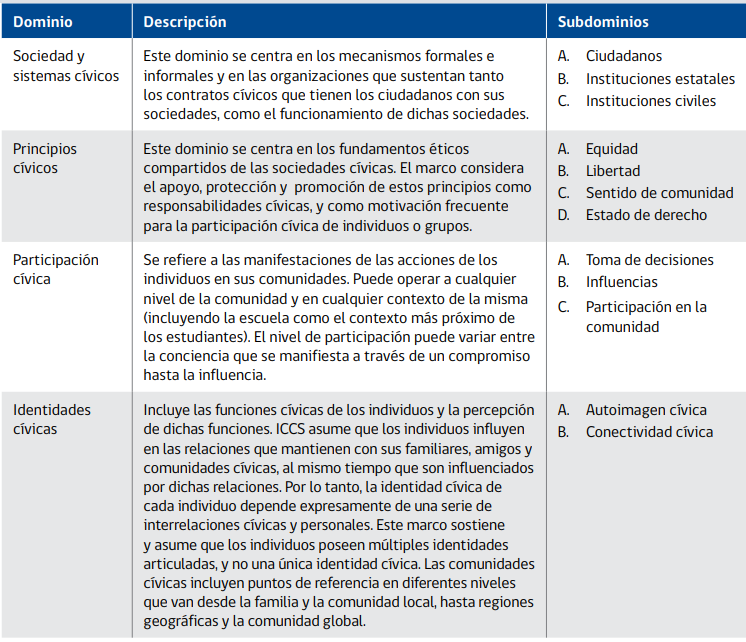
\includegraphics[width=0.8\linewidth]{images/Contenidos} \end{center}

En torno a la evidencia levantada sobre el conocimiento cívico de estudiantes medido desde la propuesta de la ICCS, se han señalado fundamentalmente dos conclusiones: primero, el conocimiento cívico posee efectos positivos en valores y conductas democráticas, y segundo, el conocimiento cívico está influido por factores contextuales como la desigualdad social y la socialización escolar.

Debido a sus efectos positivos, el conocimiento cívico y ciudadano es actualmente promovido por diversos agentes a nivel académico, Estatal e internacional. Este conocimiento es sumamente relevante si se considera sus efectos positivos sobre la intención de participación \citep{miranda_Desigualdad_2015}, en un contexto de apatía política y baja participación de estratos bajos y jóvenes \citep{janmaat_Civic_2013, contreras_DIFERENCIAS_2013}. Igualmente, en el contexto de los nuevos movimientos sociales que buscan reivindicar los derechos de distintos grupos tradicionalmente discriminados, el conocimiento cívico ha demostrado estar relacionado con el respeto a los derechos humanos de estos grupos \citep{miranda_Political_2018, caro_Ten_2012}. También, el tener más conocimiento cívico se relaciona con estar en desacuerdo con la corrupción y con la valoración positiva de la democracia como sistema representativo en contraposición a las dictaduras, lo cual, según Hastedt (2016), es fundamental en un contexto de resurgimiento de los gobiernos autoritarios. En suma, el conocimiento cívico puede ayudar a las personas a incorporar los principios democráticos de los derechos humanos.

\hypertarget{conocimiento-cuxedvico-y-desigualdad-social}{%
\subsection{Conocimiento cívico y desigualdad social}\label{conocimiento-cuxedvico-y-desigualdad-social}}

Respecto a los factores que se relacionan con distintos niveles de conocimiento cívico, destacan la influencia del nivel socioeconómico y la influencia de las prácticas democráticas en la escuela. Las investigaciones actuales han propuesto que el conocimiento cívico es especialmente influido por variables de origen socioeconómico \citep{ace_Estudio_2017, schulz_Estudio_2011, ferrans_Civic_2017, trevino_Influence_2017}, dando cuenta de lo que se denominará desde este punto, la ``Desigualdad social del conocimiento cívico''. Este efecto del nivel socioeconómico, según la literatura, se debe menos al efecto de la ocupación de los padres que al efecto de variables culturales como la educación de los padres y el número de Libros, dando luces respecto al carácter cultural del fenómeno \citep{castillo_Social_2014}. De este modo, se da cuenta del peso de la socialización familiar en el conocimiento cívico, de modo tal que criarse en un ambiente educado, probablemente con amplio vocabulario, y con acceso a recursos de aprendizaje como lo son los libros, fomenta las habilidades y conocimientos que los jóvenes necesitan para ejercer su ciudadanía en democracia´.

Además del efecto de la socialización familiar, otras investigaciones han enfatizado en el efecto producido por variables a nivel escuela como el nivel socioeconómico promedio de la escuela clima más abierto a la discusión y una cultura participativa a nivel escuela son propicios para el conocimiento cívico. En suma, podemos ver que el conocimiento cívico es influido por distintas variables que se relacionan tanto con la socialización familiar como con la escolar, destacando las variables de reproducción cultural.

En consideración de anterior, podemos decir que el conocimiento cívico es bastante explicado por el modelo de recursos, según el cual personas con mayores recursos poseen una mejor disposición a la política \citep{miranda_Desigualdad_2015}. Al explicar esta reproducción fundamentalmente cultural, la teoría de la socialización política familiar destaca dos dimensiones: la actitudinal y la cognitiva. La primera línea teórica destaca la trasmisión de valores e intereses políticos, suponiendo que convivir con padres con un mayor capital cultural conlleva tener conversaciones sobre temas políticos y sociales, que fomentan valores e intereses democráticos en los jóvenes, en contraste con la socialización apolítica de los jóvenes de estratos bajos \citep{gimpel_Cultivating_2003, wasburn_Making_2017}. La segunda, destaca la transmisión de habilidades que son heredadas por la socialización familiar en una cultura académica con lectura temprana y acceso a libros \citep{evans_Scholarly_2015, park_Home_2008}. Esta postura supone que esta cultura académica puede tener un efecto en la socialización política \citep{duarte_influence_2017, boeve-depauw_crossnational_2010}. Por su parte, la disponibilidad de libros en el hogar mejora el rendimiento académico y desarrolla habilidades mejorando con ello las habilidades para la vida política \citep{evans_Scholarly_2015}.
Además de la relevancia de los libros en el hogar existe más evidencia que hace pensar en la importancia del lenguaje y la comprensión lectora. Algunos investigadores que han realizado entrevistas cognitivas sobre la prueba de conocimiento cívico han concluido que las habilidades lingüísticas del lenguaje son relevantes para contestar exitosamente la prueba \citep{zhang_Understanding_2015, arensmeier_Swedish_2015}. En esta línea, algunos estudiantes señalaban que no comprendían la pregunta, justamente en aquellos ítems donde comprender o interpretar el sentido político es fundamental para contestar adecuadamente. De este modo se puede ver que hasta los estudiantes son relativamente consientes de la barrera interpretativa y comprensiva del lenguaje que los separa de la respuesta correcta.

En resumen, las habilidades políticas o el conocimiento cívico son un conjunto de conocimientos y habilidades necesarias para la vida ciudadana, tales como memorización de normas civicas, la interpretación y la evaluación. A partir de la evidencia, se puede sostener que estas habilidades cívicas están muy relacionadas con la socialización política familiar, en la cual influye el origen social. Al explicar esta desigualdad social de las habilidades civicas, la teoría de la socialización recurre tanto a la transmisión de actitudes como de habilidades académicas, entre las cuales esta tesis sostiene que las relativas al lenguaje son de fundamental importancia.

\hypertarget{manejo-del-lenguaje-y-comprensiuxf3n-lectora}{%
\subsection{Manejo del lenguaje y Comprensión lectora}\label{manejo-del-lenguaje-y-comprensiuxf3n-lectora}}

El lenguaje ha sido ampliamente conceptualizado a lo largo del pensamiento humano. Aristóteles, concede al lenguaje un rol elemental cuando lo concibe como la herramienta propia del \emph{zoon politikon}, ya que el lenguaje y la comunicación permite a los humanos discutir y ponerse de acuerdo. Un rol semejante le otorga al lenguaje el filósofo precursor del romanticismo Herder, cuando plantea que esta es la habilidad que da coherencia a la actividad humana, siendo una herramienta que le permite comprender la realidad y reflexionar sobre ella, a partir de conceptualizarla. Desde ambos filósofos, y desde varios otros \citep[ej.][]{echeverria_Ontologia_2011, garcia_LENGUAJE_2013}, el lenguaje es aquello que nos permite relacionarnos como humanos, usar la razón y poder discutir sobre nuestros asuntos para coexistir. Ahora bien, aunque es cierto que el lenguaje es algo propio y por ende transversal en el género humano, existe contundente evidencia para señalar que el manejo del lenguaje es diferenciado según grupos sociales.

Al respecto, el sociólogo de la línea de la reproducción cultural, Basil Berstein, realizó durante algunas décadas un amplio conjunto de experimentos e investigaciones para evaluar el uso del lenguaje en distintas clases sociales. En ellas, \citet{bernstein_CLASES_1985} concluye que los grupos económicamente acomodados y con mayores estudios, heredan a sus hijos un \emph{código sociolingüístico elaborado} del lenguaje, que les permite hacer abstracciones y pensamientos que se separan de la situación contextual en la que se encuentran. Por el contrario, los jóvenes de los barrios obreros heredan gracias al proceso de socialización un \emph{código restringido} el cual esta tendencialmente limitado a referencias contextuales y a situaciones vividas. Cabe destacar, como lo hace \citet{bernstein_Poder_1988}, que los grupos de clases medias y altas también poseen el Código restringido, pero poseen además el código elaborado el cual utilizan en situaciones desafiantes. En suma, puede evidenciarse una desigualdad sociocultural en el manejo del lenguaje que genera capacidades diferenciadas de referenciar ideas fuera de lo vivido cotidianamente, diferencias las cuales explican según el autor la desigualdad de rendimiento académico entre clases sociales, ya que el conocimiento académico se sustenta en el código elaborado, es decir, utiliza ideas fuera de la cotidianidad vivida. En suma, podemos definir al lenguaje como la base de la reflexión y la acción basada en ideas abstractas, el cual puede presentar desarrollos diferenciados socioculturalmente, lo que puede generar desigualdades en ámbitos que requieran de un lenguaje abstracto, como lo puede ser la academia o, desde esta propuesta, la política.

Un indicador útil para medir la capacidad de los estudiantes de entender distintos discursos y ser capases de comprender ideas abstractas, así como analizarlas, interpretarlas y evaluarlas, es la comprensión lectora. La comprensión lectora implica la medición de la capacidad del estudiante, no solo de decodificar el texto, sino de comprender y analizar la relación entre las distintas partes de los textos, para posteriormente realizar ejercicios mentales más complejos como los son la síntesis o la interpretación la evaluación \citep{ace_Informe_2018}. Si bien otras habilidades del manejo del lenguaje como la comprensión auditiva y la expresión escrita u oral son habilidades fundamentales para la vida política, poseen la dificultad de que es sumamente difícil medirlas de modo estandarizado. No obstante, no incorporarlas no es tan problemático considerando la amplia relación que hay entre comprender la lectura y estas otras habilidades. Para trabajar con esta variable se utilizará la prueba SIMCE, la cual, justamente busca medir los logros de aprendizaje de los estudiantes chilenos en torno a las habilidades lectoras.

Según \citet{barahonau_Factores_2014} existe un consenso en que los factores asociados al desempeño académico en lenguaje pueden tener su origen en dos grandes ámbitos: en los determinantes personales y en los determinantes sociales. Así, una de las variables fundamentales para explicar el rendimiento en lenguaje es el nivel socioeconómico según se plantea en el informe Coleman \citep{marques_Apuntes_2016}. No obstante, no todo es reproducción social, pues como plantean \citet{lara_mirada_2010}, las practicas docentes pueden tener un efecto positivo, por ejemplo, discutir la materia en clases es positivo para el rendimiento en comprensión lectora. Además de la participación en clases, el interés sobre la materia es un factor fundamental para su aprendizaje \citep{lozano_Relacion_2000}.

\hypertarget{suxedntesis-e-hipuxf3tesis.}{%
\section{Síntesis e hipótesis.}\label{suxedntesis-e-hipuxf3tesis.}}

La política y el lenguaje están altamente relacionados, de modo tal que mejores habilidades lingüísticas fomentan mejores habilidades políticas. Definimos la política como un espacio de resolución de problemas, de conflicto social y de cohesión social. Por su parte, el lenguaje fue definido como una herramienta del pensamiento humano, que permite articular individuo y sociedad, a la vez que posibilita la crítica. No obstante, como evidenciamos con las propuestas teóricas de la teoría de la reproducción cultural, las habilidades para el manejo del lenguaje se encuentran desigualmente distribuidas en la población.

En vista de lo anterior, proponemos que la reproducción intergeneracional de la desigualdad política, evidenciada en el campo de la educación cívica, puede ser explicada en cuanto a su mecanismo causal por el que opera incorporando el lenguaje como una habilidad que se transmite intergeneracionalmente y que otorga ventajas para incorporarse en la política.

En suma, el manejo del lenguaje es una habilidad que permite la reflexión, la cual es fundamental para actividades que requieren de abstracción como lo es la academia y la política. Este manejo, es adecuadamente medido por la prueba de comprensión lectora que evalúa habilidades como la comprensión, el análisis y la interpretación. Según la evidencia, el manejo del lenguaje es influido por variables socioeconómicas, por variables individuales; como el interés en la materia y por características de la escuela; como una educación participativa. Considerando la desigualdad social en el manejo del lenguaje y la complejidad del lenguaje de le prueba de conocimiento cívico, es esperable que parte de la desigualdad social del conocimiento civico se deba a las diferencias en torno al manejo del lenguaje.

En vista de las reflexiones y evidencias anteriores se proponen las siguientes hipótesis.

\begin{itemize}
\item
  \(H_1\) Existe \emph{desigualdad social del conocimiento cívico}, es decir, los estudiantes de familias con mayor nivel socioeconómico poseen un mayor nivel conocimiento cívico.
\item
  \(H_2\) El manejo del lenguaje posee un efecto positivo sobre el conocimiento cívico del estudiante.
\item
  \(H_3\) El manejo del lenguaje media parcialmente la relación del estatus ocupacional y educacional de los padres sobre el conocimiento cívico del estudiante.
\item
  \(H_4\) El manejo del lenguaje media totalmente la relación entre cantidad de libros en el hogar y el conocimiento cívico del estudiante.
\end{itemize}

\begin{figure}

{\centering 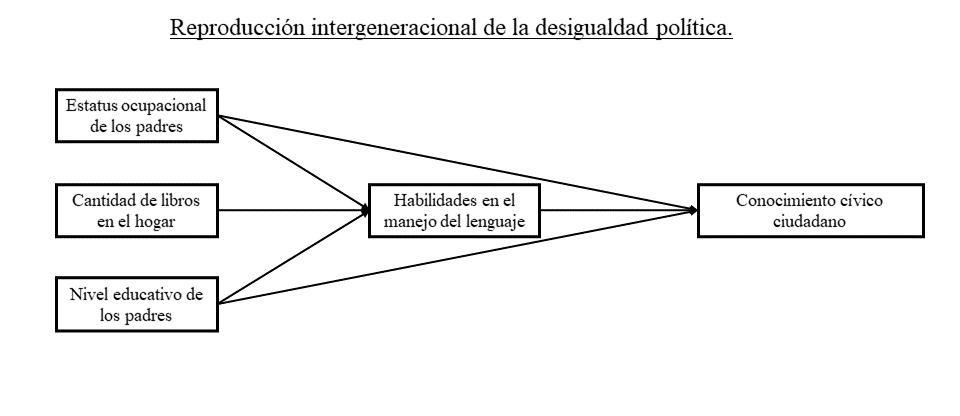
\includegraphics[width=0.95\linewidth]{images/modelo} 

}

\caption{Modelo teórico}\label{fig:unnamed-chunk-2}
\end{figure}

Junto con lo anterior, y considerando la capacidad positiva del colegio de mejorar la comprensión lectora de sus estudiantes mediante buenas prácticas como la discusión en clase y la motivación de sus estudiantes, se propone que el colegio puede fomentar un manejo del lenguaje que supere el efecto de la familia, lo cual podría moderar las desigualdades sociales del conocimiento cívico.

\begin{itemize}
\tightlist
\item
  \(H_5\) El manejo del lenguaje es capaz de moderar el efecto del nivel socioeconómico sobre el conocimiento cívico.
\end{itemize}

\hypertarget{metodologuxeda}{%
\chapter{Metodología}\label{metodologuxeda}}

\hypertarget{datos}{%
\section{Datos}\label{datos}}

\hypertarget{iccs}{%
\subsection{ICCS}\label{iccs}}

Para abordar la pregunta de investigación se trabajará con la base de datos de la encuesta internacional de conocimiento cívico (ICCS) en su tercera versión (2016). La ICCS es una encuesta enfocada en el estudio longitudinal del conocimiento cívico y las actitudes democráticas en estudiantes de octavo grado de 24 países. Dieciséis de esos países son de Europa, cinco de América Latina y tres de Asia, representados por 94.000 estudiantes y 37.000 profesores de 3.800 colegios \citep{schulz_ICCS_2016}. Junto con una estrecha colaboración entre la IEA y los centros de estudios de cada país, los encargados de la elaboración de los datos fueron El Consejo Australiano para la Investigación Educativa (ACER) en Melbourne y el Laboratorio di Pedagogia Sperimentale (LPS) en la Universidad Roma Tre \citep{iea_International_2016}. La muestra de estudiantes posee un diseño estratificado de dos etapas, eligiendo escuelas al azar en un país y aulas al azar en una escuela, de tal modo que cada país tenga aproximadamente 150 escuelas y entre 3000 y 45000 estudiantes. La muestra de chile, con trabajo de campo en el 2015, incorporo colegios elegidos aleatoriamente, y representativos de distintas dependencias y regiones, tanto de sectores rurales como urbanos. De las escuelas seleccionadas aleatoriamente el 85\% acepto participar, y dentro de las escuelas participantes, el 85\% de los estudiantes acepto participar. En total, participaron 5.081 estudiantes de 178 establecimientos según señala la agencia de calidad de la educación \citep{ace_Informe_2018a}.

\hypertarget{simce}{%
\subsection{SIMCE}\label{simce}}

Adicionalmente se utilizaron los datos Simce del 2015, prueba censal que fue aplicada a los mismos estudiantes participantes del estudio de la ICCS, lo cual permite agregar estas bases de datos, logrando tener las variables de ambos estudios para cada estudiante de la muestra del ICCS. El Simce evalúa los logros de aprendizaje en las asignaturas de Lenguaje y Comunicación (Comprensión Lectura y Escritura); Matemática; Ciencias Naturales; Historia, Geografía y Ciencias Sociales e Inglés. En esta ocasión, hemos utilizado los datos de la prueba Simce de lenguaje y comunicación, más específicamente, de comprensión lectora. El estudio Simce, al igual que el ICCS, trabaja con el modelo de medición de ITR (Teoria de respuesta al ítem). ``En particular {[}el Simce trabaja con{]} el modelo IRT de tres parámetros, {[}el cual{]} permite estimar la habilidad de un estudiante, basándose en la probabilidad de respuesta correcta según tres características propias de las preguntas: dificultad, discriminación y azar \citep{ace_Informe_2018}. Los procesos de aplicación de los instrumentos (pruebas y cuestionarios10) se llevan a cabo en función de instrucciones, manuales y protocolos de actuación que se basan en los criterios de estandarización internacional \citep{aera_Report_2011}.

Respecto al tipo de preguntas, estas son de opción múltiple, pues este formato permite reportar información de la mayoría de los constructos a evaluar en forma efectiva y eficiente, asegurando validez, confiabilidad y objetividad del instrumento en su totalidad \citep{rupp_Handbook_2008}. En miras de este objetivo de la validez del instrumento, se realizan desde el año anterior a la aplicación pruebas piloto, las cuales son analizadas cualitativa y cuantitativamente para construir los indicadores más adecuados posibles. En suma, el Simce realiza una Logística de preparación que implica un gran gasto de recursos con el objetivo de reducir al máximo el error de medida.

\hypertarget{variables}{%
\section{Variables}\label{variables}}

\hypertarget{prueba-de-conocimiento-cuxedvico-y-ciudadano}{%
\subsection{Prueba de conocimiento cívico y ciudadano}\label{prueba-de-conocimiento-cuxedvico-y-ciudadano}}

La prueba de conocimiento cívico de la ICCS tiene como objetivo evaluar los conocimientos necesarios para comprender y valorar la vida en sociedad y las formas de organización democrática, la capacidad de razonar acerca de las instituciones, eventos, acciones y procesos que se desarrollan en sus comunidades y la habilidad de desarrollar y justificar opiniones y visiones sobre estos elementos \citep{schulz_Initial_2010}. Los ítems de prueba requerían que los estudiantes aplicaran los procesos cognitivos al contenido cívico y de ciudadanía como se describe en el marco de evaluación del reporte técnico \citep{schulz_ICCS_2016}. Más específicamente, la prueba de conocimiento Cívico y ciudadano mide:

\begin{itemize}
\tightlist
\item
  \emph{Dominios de contenido}

  \begin{itemize}
  \tightlist
  \item
    Sociedad y sistemas cívicos
  \item
    principios cívicos
  \item
    Participación cívica
  \item
    Identidades cívicas
  \end{itemize}
\item
  \emph{Dominios cognitivos}

  \begin{itemize}
  \tightlist
  \item
    conocimiento memorización
  \item
    Razonamiento y aplicación
  \end{itemize}
\end{itemize}

Se utilizaron dos formatos de ítems: 79 de 88 ítems de la prueba son de opción múltiple con cuatro opciones de respuesta, como se puede ver en los ejemplos de los Anexos; los nueve ítems restantes fueron de respuesta construida para los cuales los estudiantes debían escribir entre una y tres oraciones. Para calcular los puntajes de cada estudiante, se parte de una media de 500 puntos, considerando una desviación estándar de 100 puntos, y según esta métrica se calculan 5 posibles resultados para cada estudiante. El que sean 5 resultados refleja el error y la incertidumbre propia de la medición de constructos complejos, al respecto se ha decidido trabajar con la primera estimación de puntaje. Según el reporte técnico \citep{schulz_ICCS_2016}, se utilizó la teoría de respuesta al ítem. Para escalar los datos de prueba de ICCS 2016, los autores recurrieron al paquete de software de escalado ACER ConQuest, Versión 4. Posteriormente se realizaron diversas pruebas de validez, confiabilidad y equivalencia para comprobar que el conocimiento cívico es un constructo unidimensional, continuo y fiable.
Además de las evaluaciones de fiabilidad, invarianza, equivalencia y validez realizadas por los centros de investigación designados por la IEA en el marco de la ICCS, otras agencias han evaluado la calidad de los cuestionarios. Así, por ejemplo, la agencia nacional de educación, evaluar el sesgo de deseabilidad social, concluyendo que la prueba no presenta problemas mayores de deseabilidad, y que estos se concentran en los aspectos de preguntas de actitudes y opiniones (Mineduc, 2019).

A continuación, se presenta una tabla con distintos rangos de puntaje y distintas capacidades que son asociadas a este puntaje. Como puede verse seria optimo que los jóvenes alcancen puntajes de conocimiento cívico superiores a 563 puntos.

\begin{figure}

{\centering 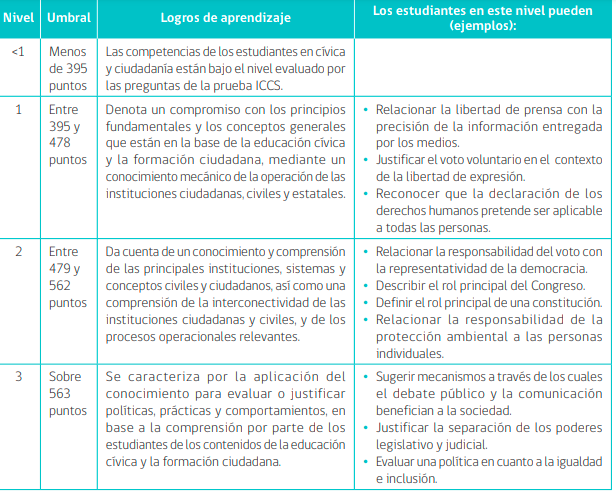
\includegraphics[width=0.8\linewidth]{images/puntajesdecorteiccs} 

}

\caption{Rangos ICCS}\label{fig:unnamed-chunk-3}
\end{figure}

Cabe destacar, que esta prueba de conocimiento cívico ya ha pasado por tres olas internacionales, a partir de las cuales se ha refinado las características psicométricas de la medición. Esta prueba consta tanto de preguntas de selección múltiple como preguntas abiertas, a continuación, se presenta un ejemplo de pregunta en la cual se miden dominios cognitivos de razonamiento y análisis. Al respecto es importante destacar como esta pregunta requiere tanto de conocimientos políticos, como de habilidades propias del lenguaje como es la interpretación. Al respecto, \citet{schulz_Estudio_2011}, señalan que las preguntas de razonamiento y análisis requieren del uso del lenguaje para interpretar información, relatar, justificar, integrar, generalizar, evaluar, sugerir soluciones o predecir.

\begin{figure}

{\centering 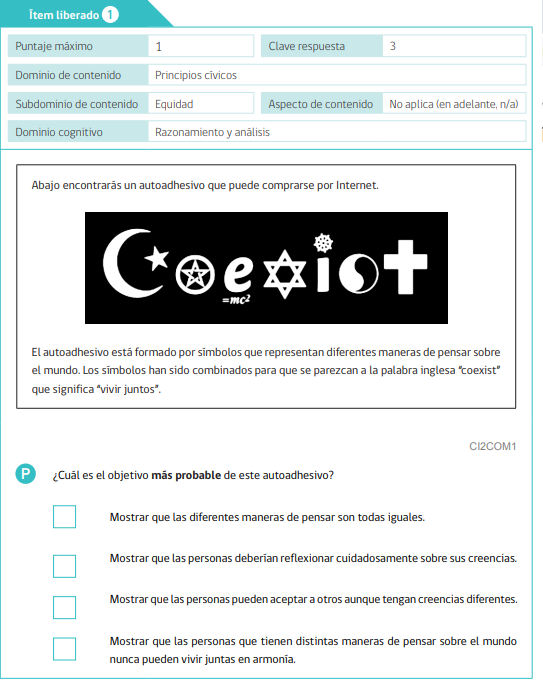
\includegraphics[width=0.8\linewidth]{images/Pregunta-liberada1} 

}

\caption{Pregunta ejemplo ICCS}\label{fig:unnamed-chunk-4}
\end{figure}

\hypertarget{prueba-de-comprensiuxf3n-lectora}{%
\subsection{Prueba de comprensión lectora}\label{prueba-de-comprensiuxf3n-lectora}}

La comprensión lectora busca evaluar a los estudiantes en su capacidad de manejo del lenguaje y la comunicación. Específicamente, la prueba de lenguaje evalúa las siguientes actividades.

\begin{itemize}
\tightlist
\item
  Localizar información

  \begin{itemize}
  \tightlist
  \item
    Identificar
  \item
    Discriminar
  \item
    Extraer
  \end{itemize}
\item
  Interpretar

  \begin{itemize}
  \tightlist
  \item
    Inferir
  \item
    Interpretar lenguaje denotativo
  \item
    Reconocer relaciones causales
  \end{itemize}
\item
  Reflexionar

  \begin{itemize}
  \tightlist
  \item
    Contrastar con conocimientos previos
  \item
    Evaluar críticamente aspecto de contenido y formato
  \end{itemize}
\end{itemize}

Así, como puede apreciarse, para un buen puntaje en comprensión lectora, no solo se requiere la capacidad de decodificar el significado de las palabras, sino que se requiere un manejo del lenguaje a un nivel de razonamiento. Como ya se comentó, el proceso de elaboración y aplicación de la prueba tiene el objetivo de disminuir al mínimo variables externas al manejo del lenguaje que pudieran afectar la medición. Para evaluar las propiedades psicométricas de esta prueba, los encargados de la prueba Simce realizaron análisis en base a lineamientos internacionales \citep{aera_Report_2011}. En base a los análisis realizados por el equipo técnico \citep{ace_Informe_2018}, podemos decir que la prueba de comprensión lectora es unidimensional (i.e El AFC indica un solo factor), posee independencia local (i.e estudiantes de un mismo rendimiento no presentan dificultades para determinada pregunta por factores externos) y motricidad creciente (i.e es un constructo continuo donde la probabilidad de responder correctamente un ítem aumenta progresivamente en estudiantes de mayor rendimiento).

\begin{figure}

{\centering 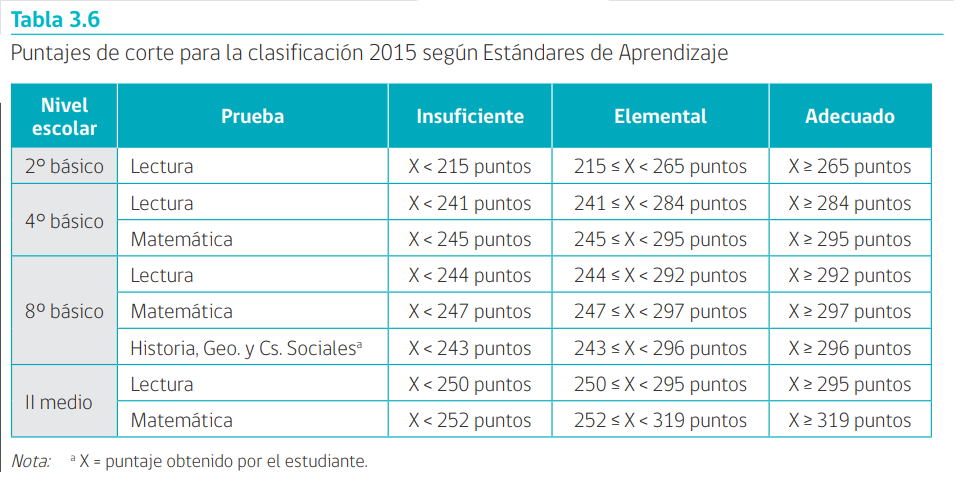
\includegraphics[width=0.8\linewidth]{images/Rangos-puntaje-simce} 

}

\caption{Rangos Simce}\label{fig:unnamed-chunk-5}
\end{figure}

\hypertarget{estatus-socioeconuxf3mico-del-estudiante-y-del-colegio.}{%
\subsection{Estatus socioeconómico del estudiante y del colegio.}\label{estatus-socioeconuxf3mico-del-estudiante-y-del-colegio.}}

Para trabajar la medicación del estatus socioeconómico del colegio, se trabajará con tres variables, el estatus ocupacional más alto entre los padres, el nivel educativo más alto de los padres y la cantidad de libros en el hogar. Para simplificar los cálculos a realizar, las dos últimas variables serán dicotomizadas de tal modo que representen, tener un padre con educación universitaria y poseer más de 100 libros en el hogar respectivamente. Dicotomizar las variables permitirá disminuir la cantidad de parámetros a estimar y la existencia de categorías con muy pocas respuestas en las escuelas las cuales sestan altamente segregadas socioeconómicamente. Estas variables serán utilizadas para trabajar la mediación.

Para trabajar la moderación del efecto del nivel socioeconómico de los estudiantes se utilizará el Índice nacional de antecedentes socioeconómicos el cual es elaborado por el equipo de la encuesta ICCS. Este índice es elaborado como un puntaje factorial que representa una variable latente relacionada con el mayor nivel ocupacional entre los padres, el mayor nivel educativo entre los padres y la cantidad de libros declarados en el hogar. Para evaluar el contexto socioeconómico del establecimiento educativo, se trabajará con el promedio por colegio del Índice nacional de antecedentes socioeconómicos.

\hypertarget{variables-de-control}{%
\subsection{Variables de control}\label{variables-de-control}}

Para medir el interés político los estudiantes se utilizará la pregunta creada por la encuesta internacional ICCS. En este ítem se le pregunta al estudiante ¿Qué tan interesado está en temas políticos y sociales? (Muy interesado/ Bastante interesado / No muy interesado / No me interesa en absoluto). Para simplificar el análisis se ha recodificado esta pregunta de tal modo que las dos primeras alternativas se resumen en ``Interesado en la politica'' y las últimas dos en ``No interesado en la política''. Cabe destacar que, para el análisis de mediación, se utilizó la variable original de 4 categorías centrada al promedio de la escuela.

Además, como variables de control, será incluida la calidad de la discusión en el aula, ya que este es un indicador que ha sido consistentemente señalado como relevante por la evidencia, esta variable de nivel dos corresponde al promedio de los indicadores relacionados con las preguntas de clima en el aula.

\hypertarget{muxe9todos}{%
\section{Métodos}\label{muxe9todos}}

Respecto al método, este estudio trabajara desde un enfoque cuantitativo transversal. El uso de las herramientas cuantitativas es fundamental para despejar las dudas planteadas en este artículo, puesto que la cuantificación, como medición de lo social \citep{canales_METODOLOGIAS_2006}, nos permitirá contrastar que variable posee una mejor capacidad mediadora de la reproducción de la desigualdad política, la comprensión lectora o el interés político. A continuación, se hace una exposición de las técnicas con las que se trabajara y se explicara por qué son indispensables para abordar la temática.

El centro del trabajo utilizara estadística multivariada, más particularmente, regresiones lineales. Las regresiones lineales según Hayes poseen la intención evaluar la capacidad predictiva de una variable sobre otra. Para representar la relación gráfica y numéricamente, se busca restimar una línea que represente la relación entre una variable independiente y una dependiente. Esta línea se superpone a un gráfico de dispersión en el cual cada caso s situado en una posición según su valor en el eje x y el eje ``y''. De este modo, cuando no hay relación se forma una nube dispersa, mientras que más es la relación los puntos se ajustan más a una línea. La regresión nos permite encontrar la línea que mejor representa la relación. Esta línea en un plano cartesiano nos permite tener conclusiones del tipo ``mientras más se tiene de esta variable más se tiene de esta otra''. Para llegar a estimar esa línea que representa mejor la relación se utiliza la técnica de mínimos cuadrados, la cual es un proceso iterativo donde a partir de probar múltiples rectas, se evalúa cuál de ellas genera la menor cantidad de residuos. Los residuos corresponden a la varianza de la dependiente que no es explicada por la independiente. Si dos variables están completamente relacionadas no habrá residuos, y la línea pasará por cada uno de los puntos del gráfico. Matemáticamente, esto implica que el valor de los casos en el plano restado a el valor predicho es 0. Se realiza un cálculo que busca encontrar la recta que genera el mínimo, de residuos y por ende, representa mejor la relación, que se supone lineal.

Las relaciones pueden ser positivas o negativas. Cuando una relación es positiva se ve que la línea que mejor representa la relación parte al comienzo del grafico en la izquierda en un valor menor y que aumenta en tanto avanza a la derecha. Una relación negativa por el contrario implica que a mayor valor de x menor valor de y.

Los parámetros entregados por la regresión son, p de significación, betas que representan la relación, r2 que representan la fuerza de la relación y un intercepto, el cual corresponde al promedio en un modelo sin predictores y aumenta o disminuye según se incline la línea de predicción. Por ende, el intercepto puede ser interpretado como el corte con el eje y cuando la variable dependiente está en 0, lo cual no siempre tiene una aplicación directa.

Las ventajas de las regresiones son múltiples. En primer lugar, como medida de relación cumple con las exigencias señalada por la metodología. Posee un valor por qué nos permite evaluar si es posible extrapolar las conclusiones al universo. Este valor p representa la posibilidad de que la pendiente sea efectivamente distinta a 0, es decir, la posibilidad de que no exista relación. Además, siguiendo los consejos de Cohen, las regresiones entregan un valor que indica la fuerza de la relación lo cual es fundamental para comprender la magnitud de los fenómenos que estamos evaluando.

Una segunda ventaja de las regresiones líneas para nuestro trabajo es que permiten realizar control estadístico. El control estadístico es un proceso complejo por el cual mediante la parcialización de los efectos se puede despejar los efectos comunes de dos variables, para evaluar cual es efectivamente la que posee una influencia sobre la dependiente. De este modo, siguiendo con nuestras hipótesis, el efecto que es generado inicialmente por el nivel socioeconómico debería poder ser controlado por el efecto del manejo del lenguaje, por qué en última instancia las diferencias deben al mejor manejo del lenguaje en los niveles socioeconómico más altos. Otra forma de entender el control estadístico es considerar los efectos controlados como el efecto de una variable cuando la otra está constantemente en 0.

El control estadístico se logra a partir del proceso de parcialización el cual corresponde a explicar una independiente por otra independiente, y eliminar todo aquello que es explicado (varianza compartida) utilizando los residuos de esa regresión como variable independiente.

Se trabajará con técnicas de regresión multinivel, ya que estas son indispensables al estudiar muestras jerárquicas de colegios. Las regresiones multinivel, a diferencia de las regresiones normales, asumen que los estudiantes de un mismo establecimiento compartirán características debido al contexto común. Si se trabajara con regresiones lineales de un solo nivel, se rompería el supuesto de independencia de los casos en la muestra, ya que los casos están relacionados entre sí al pertenecer a los mismos establecimientos. Esta metodología también nos permite evaluar el efecto de características de la escuela, como lo son el NSE promedio o la percepción promedio de apertura a la discusión. Más específicamente, dentro del trabajo con regresiones multinivel, se trabajará con relaciones pendientes aleatorias, mediación multinivel e interacciones entre niveles.

Para entender el concepto de multinivel y su operación estadística es necesario primero comprender la idea de varianza entre y dentro. Pensemos en comprensión lectora. Es sabido que existen colegios que poseen una mejor comprensión lectora que otros. Este efecto no se debe particularmente a que cada uno de los niños, sino que se puede deber a que el colegio posee una mejor educción o a que es más selectivo. De este modo se puede ver que hay varianza entre los estudiantes que corresponde a la varianza entre los colegios. Es el efecto de pertenecer a un mejor colegio que otro. Por otro lado, además de esas diferencias entre colegios hay diferencias dentro de los colegios. Entre estudiantes de un liceo de mal desempeño, existen estudiantes mejores que otros y algunos que pueden sobresalir. En alguna medida, se puede esperar que estas diferencias dentro de las escuelas sean producto del esfuerzo del niño o de los apoyos y ventajas que les ofrecen sus padres.

Con esa distinción conceptual en mente, veamos que hacen las regresiones multinivel. Para ello es necesario comprender que estas regresiones consideran los grupos en los cuales esta cada sujeto, en este caso las escuelas. Estadísticamente diferencian los residuos de la varianza, en residuos entre colegios y residuos dentro de los colegios. Cuando una variable a nivel escuela como la calidad de los profesores afecta la variable dependiente, esta reducirá los residuos entre colegios. Por su parte, cuando se tiene una variable individual que afecta las diferencias entre los niños, como poseer profesores particulares, esto disminuirá la varianza dentro de las escuelas.

Para la existencia de los residuos diferenciados, es necesaria la estimación de dos tipos de líneas de regresión. La primera es una pendiente general que representa la relación a nivel 2. El segundo tipo de línea, son las pendientes en cada grupo. Esta diferencia permite la variación de los parámetros entre los grupos. De este modo, se pueden agregar dos parámetros muy interesantes. Un intercepto aleatorio y una pendiente aleatoria. El termino aleatorio no refiere a que es azaroso, sino que varia entre grupos.\\
La variación de los intercepto nos indica cuando dieren los intercepto entre los grupos. El intercepto aleatorio nos puede indicar que en algunos establecimientos el nivel de conocimiento cívico (variable y) es mayor ante el valor mínimo de manejo del lenguaje (variable x)
Las pendientes aleatorias sirven para evaluar como varia la pendiente de una relación en distintos contextos, para este trabajo se calculará la variación de la pendiente de la relación entre conocimiento cívico y comprensión lectora.

La medición multinivel permite evaluar una cadena causal considerando la estructura jerárquica de los datos. Para comprender esta metodología, es necesario entender que una medicación corresponde al fenómeno según el cual una variable ``X'', explica una variable ``Y'', por medio de ``M'', de tal modo que ``X'' genera ``M'' y M genera ``Y'' \citep{mathieu_framework_2007}. Al igual que en una mediación de un solo nivel, es requisito para comprobar la mediación multinivel, que ``X'' sea capaz de explicar tanto ``M'' como ``Y'', y que, además, M sea capaz de explicar ``Y'', controlando, en alguna medida el efecto de ``X'' \citep{baron_moderator_1986}. Existen distintos tipos de análisis de mediación cuando se trabaja con lógicas multinivel. Se puede hablar de mediaciones intra-niveles que solo involucran una mediación dentro del Nivel 1 o Nivel 2, y también se puede hablar de meso-mediaciones, en las cuales la mediación pasa de un nivel a otro \citep{mathieu_framework_2007}. En nuestro caso, contamos con una mediación intra-nivel, ya que todas las variables involucradas en la mediación son de nivel 1, aunque sea relevante considerar y controlar por características de Nivel 2 ya que los datos están anidados. En nuestro caso, queremos evaluar la capacidad de la comprensión lectora de mediar la relación entre NSE y conocimiento cívico, por ende, debemos evaluar la capacidad explicativa del NSE sobre la comprensión lectora y el conocimiento cívico (CC), y posteriormente, ver la capacidad del manejo del lenguaje de controlar el efecto del NSE sobre CC.

Considerando las recomendaciones de \citep{zhang_Testing_2009} para cuando todas las variables del proceso de mediación se encuentran en el primer nivel, es fundamental, para evitar confusiones de los efectos producidas por la estructura jerárquica de la muestra, evaluar las relaciones en ambos niveles, es decir, un efecto de mediación intragrupo y otro entre grupos, para ello se deben realizar centrados en las medias de los grupos, según concluyeron los investigadores a partir de pruebas de simulación Montecarlo.

Esta propuesta si bien será utilizada y es muy enriquecedora metodológicamente, posee dos limitaciones que es necesario resolver para poder trabajar rigurosamente nuestras hipótesis. En primer lugar, esta forma de trabajar las relaciones multinivel no permite saber si el efecto indirecto es significativo, como Sobel señala necesario. Por ello para subsanar esta falencia se utilizará la prueba de Sobel. En segundo lugar, esta perspectiva tampoco permite abordar los tamaños de efecto, por lo cual se considera necesario incluir el efecto mediado en términos de R2, para lo cual se recurrirá a la estimación de Bryk \& Raudenbusch (1992).

A continuación, se expone el cálculo que a realizar para probar la mediación multinivel. En general el modelo señala que el Conocimiento cívico es explicado por la comprensión lectora, la cual a su vez se debe a los recursos de la familia. El modelo también calcula los efectos directos e indirectos de los recursos de la familia sobre el conocimiento cívico. Las siguientes formulas no contienen todos los controles señalados.

\begin{enumerate}
\def\labelenumi{\alph{enumi})}
\tightlist
\item
  \emph{Influencia de los recursos familiares en el lenguaje}
\end{enumerate}

\begin{equation}
\text{C.Lectora}= i_1 +\gamma_{10}\text{Ocupación}_{ij} + \gamma_{20}\text{Universitarios}_{ij}+ \gamma_{30}\text{Libros}_{ij}+u_{0j}+r_{ij}
\end{equation}

\begin{enumerate}
\def\labelenumi{\alph{enumi})}
\setcounter{enumi}{1}
\tightlist
\item
  \emph{Influencia directa de los recursos familiares en lo cívico}
\end{enumerate}

\begin{equation}
\text{C.Civico}= i_2+\gamma_{40}\text{Ocupación}_{ij} + \gamma_{50}\text{Universitarios}_{ij}+ \gamma_{60}\text{Libros}_{ij}+u_{0j}+r_{ij}
\end{equation}

\begin{enumerate}
\def\labelenumi{\alph{enumi})}
\setcounter{enumi}{2}
\tightlist
\item
  \emph{Influencia del lenguaje e influencia controlada de los recursos familiares en lo cívico}
\end{enumerate}

\begin{equation}
\text{C.Civico}= i_+\gamma_{70}\text{C.Lectora}_{ij}+\gamma_{70}\text{Ocupación}_{ij} + \gamma_{80}\text{Universitarios}_{ij}+ \gamma_{90}\text{Libros}_{ij}+u_{0j}+r_{ij}
\end{equation}

\begin{itemize}
\item
  Efectos indirectos de recursos familiares sobre conocimiento cívico

  \begin{itemize}
  \item
    Ocupación de los padres = \(\gamma_{10}\times\gamma_{70}\)
  \item
    Padres Universitarios = \(\gamma_{20}\times\gamma_{80}\)
  \item
    Libros en el hogar = \(\gamma_{30}\times\gamma_{90}\)
  \end{itemize}
\end{itemize}

En suma, se evaluará la medicación de la comprensión lectora sobre la relación entre NSE y conocimiento Cívico, evaluando la relación a nivel dos y a nivel uno, incorporando centrados a la media del grupo. Se espera que el efecto de NSE sobre CC disminuya en buena medida al incluir el control de la comprensión lectora. además, se espera que la disminución del efecto por control sea mayor al incluir la variable comprensión lectora que interés político.

En términos de interacciones entre niveles, evaluaremos la capacidad de la comprensión lectora del estudiante de moderar el efecto negativo sobre el conocimiento cívico que se debería de pertenecer a un establecimiento de bajo NSE promedio. Siguiendo las buenas prácticas para interacciones multinivel propuestas por \citep{aguinis_BestPractice_2013}, se centraron las variables según el promedio de la escuela, con la intención de despejar debidamente el componente individual de la varianza.

\hypertarget{software}{%
\subsection{Software}\label{software}}

El software de análisis estadístico utilizado fue R (versión 4.02) y la plataforma de edición GitHub. Para los análisis multinivel recurrimos al paquete lme4, en su versión 1.1-23 \citep{bates_Package_2020}.

Además, siguiendo los lineamientos de la ciencia abierta, este trabajo está en un repositorio para facilitar tanto su acceso como su reproductibilidad. El lector de este seminario esta cordialmente invitado a visitar la \href{https://franciscomeneses.github.io/Seminario/docs/index.html}{página web del proyecto} en la que se puede revisar tanto el articulo como los análisis. Igualmente, si el lector desea reproducir los análisis para verificar su veracidad, puede descartar el proyecto desde el \href{https://github.com/franciscomeneses/Seminario}{repositorio de Github}. Para facilitar la comprensión del orden de los archivos, estos se han ordenado según el esquema \href{https://juancarloscastillo.github.io/ipo/}{IPO}, propuesto por Castillo (2020)

\hypertarget{anuxe1lisis}{%
\chapter{Análisis}\label{anuxe1lisis}}

A continuación, se presentan análisis uni y bivariados para las variables más importantes del estudio. De este modo buscamos aproximarnos a la realidad del país para sacar mejores conclusiones en torno a los modelos. De este modo, podremos comprender los actuales niveles de conocimiento cívico y comprensión lectora de nuestros estudiantes. Para los análisis descriptivos, bivariados y multivariados, se utilizan los puntos de corte del conocimiento cívico y de la comprensión lectora señalados respectivamente por el Mineduc y los representantes de la IEA. Los puntos de corte ayudaran a comprender la magnitud de las diferencias y las reales implicancias de la temática.

\hypertarget{anuxe1lisis-descriptivo}{%
\section{Análisis descriptivo}\label{anuxe1lisis-descriptivo}}

El presente gráfico presenta la distribución del conocimiento cívico en los estudiantes chilenos de octavo básico del 2015. Junto a la distribución se expone el porcentaje de estudiantes que se encuentra en cada nivel del conocimiento cívico. Como se puede ver en la imagen casi un 15\% de los estudiantes se encuentra por debajo del nivel que pretende medir la prueba de la ICCS, lo cual es un dato bastante preocupante. Seguidamente un cuarto de los estudiantes posee conocimientos cívicos y algún compromiso con valores democráticos, pero no comprende el funcionamiento de las principales instituciones. Un tercio de los estudiantes si comprende los conceptos más relevantes y es capaz de comprender la interacción de las distintas instituciones cívicas y ciudadanas en procesos relevantes, pero no es capaz de aplicar estos conocimientos para evaluar situaciones concretas. Finalmente, la cuarta parte de los estudiantes alcanzan el máximo nivel señalado por la ICCS, denotando ser capases de aplicar estos conocimientos para evaluar o justificar situaciones concretas. Cabe destacar que el promedio de los estudiantes bordea los 500 puntos, estando en el nivel de compresión, además el puntaje mínimo es 232,1 y el puntaje máximo es 782,7.

\begin{figure}

{\centering 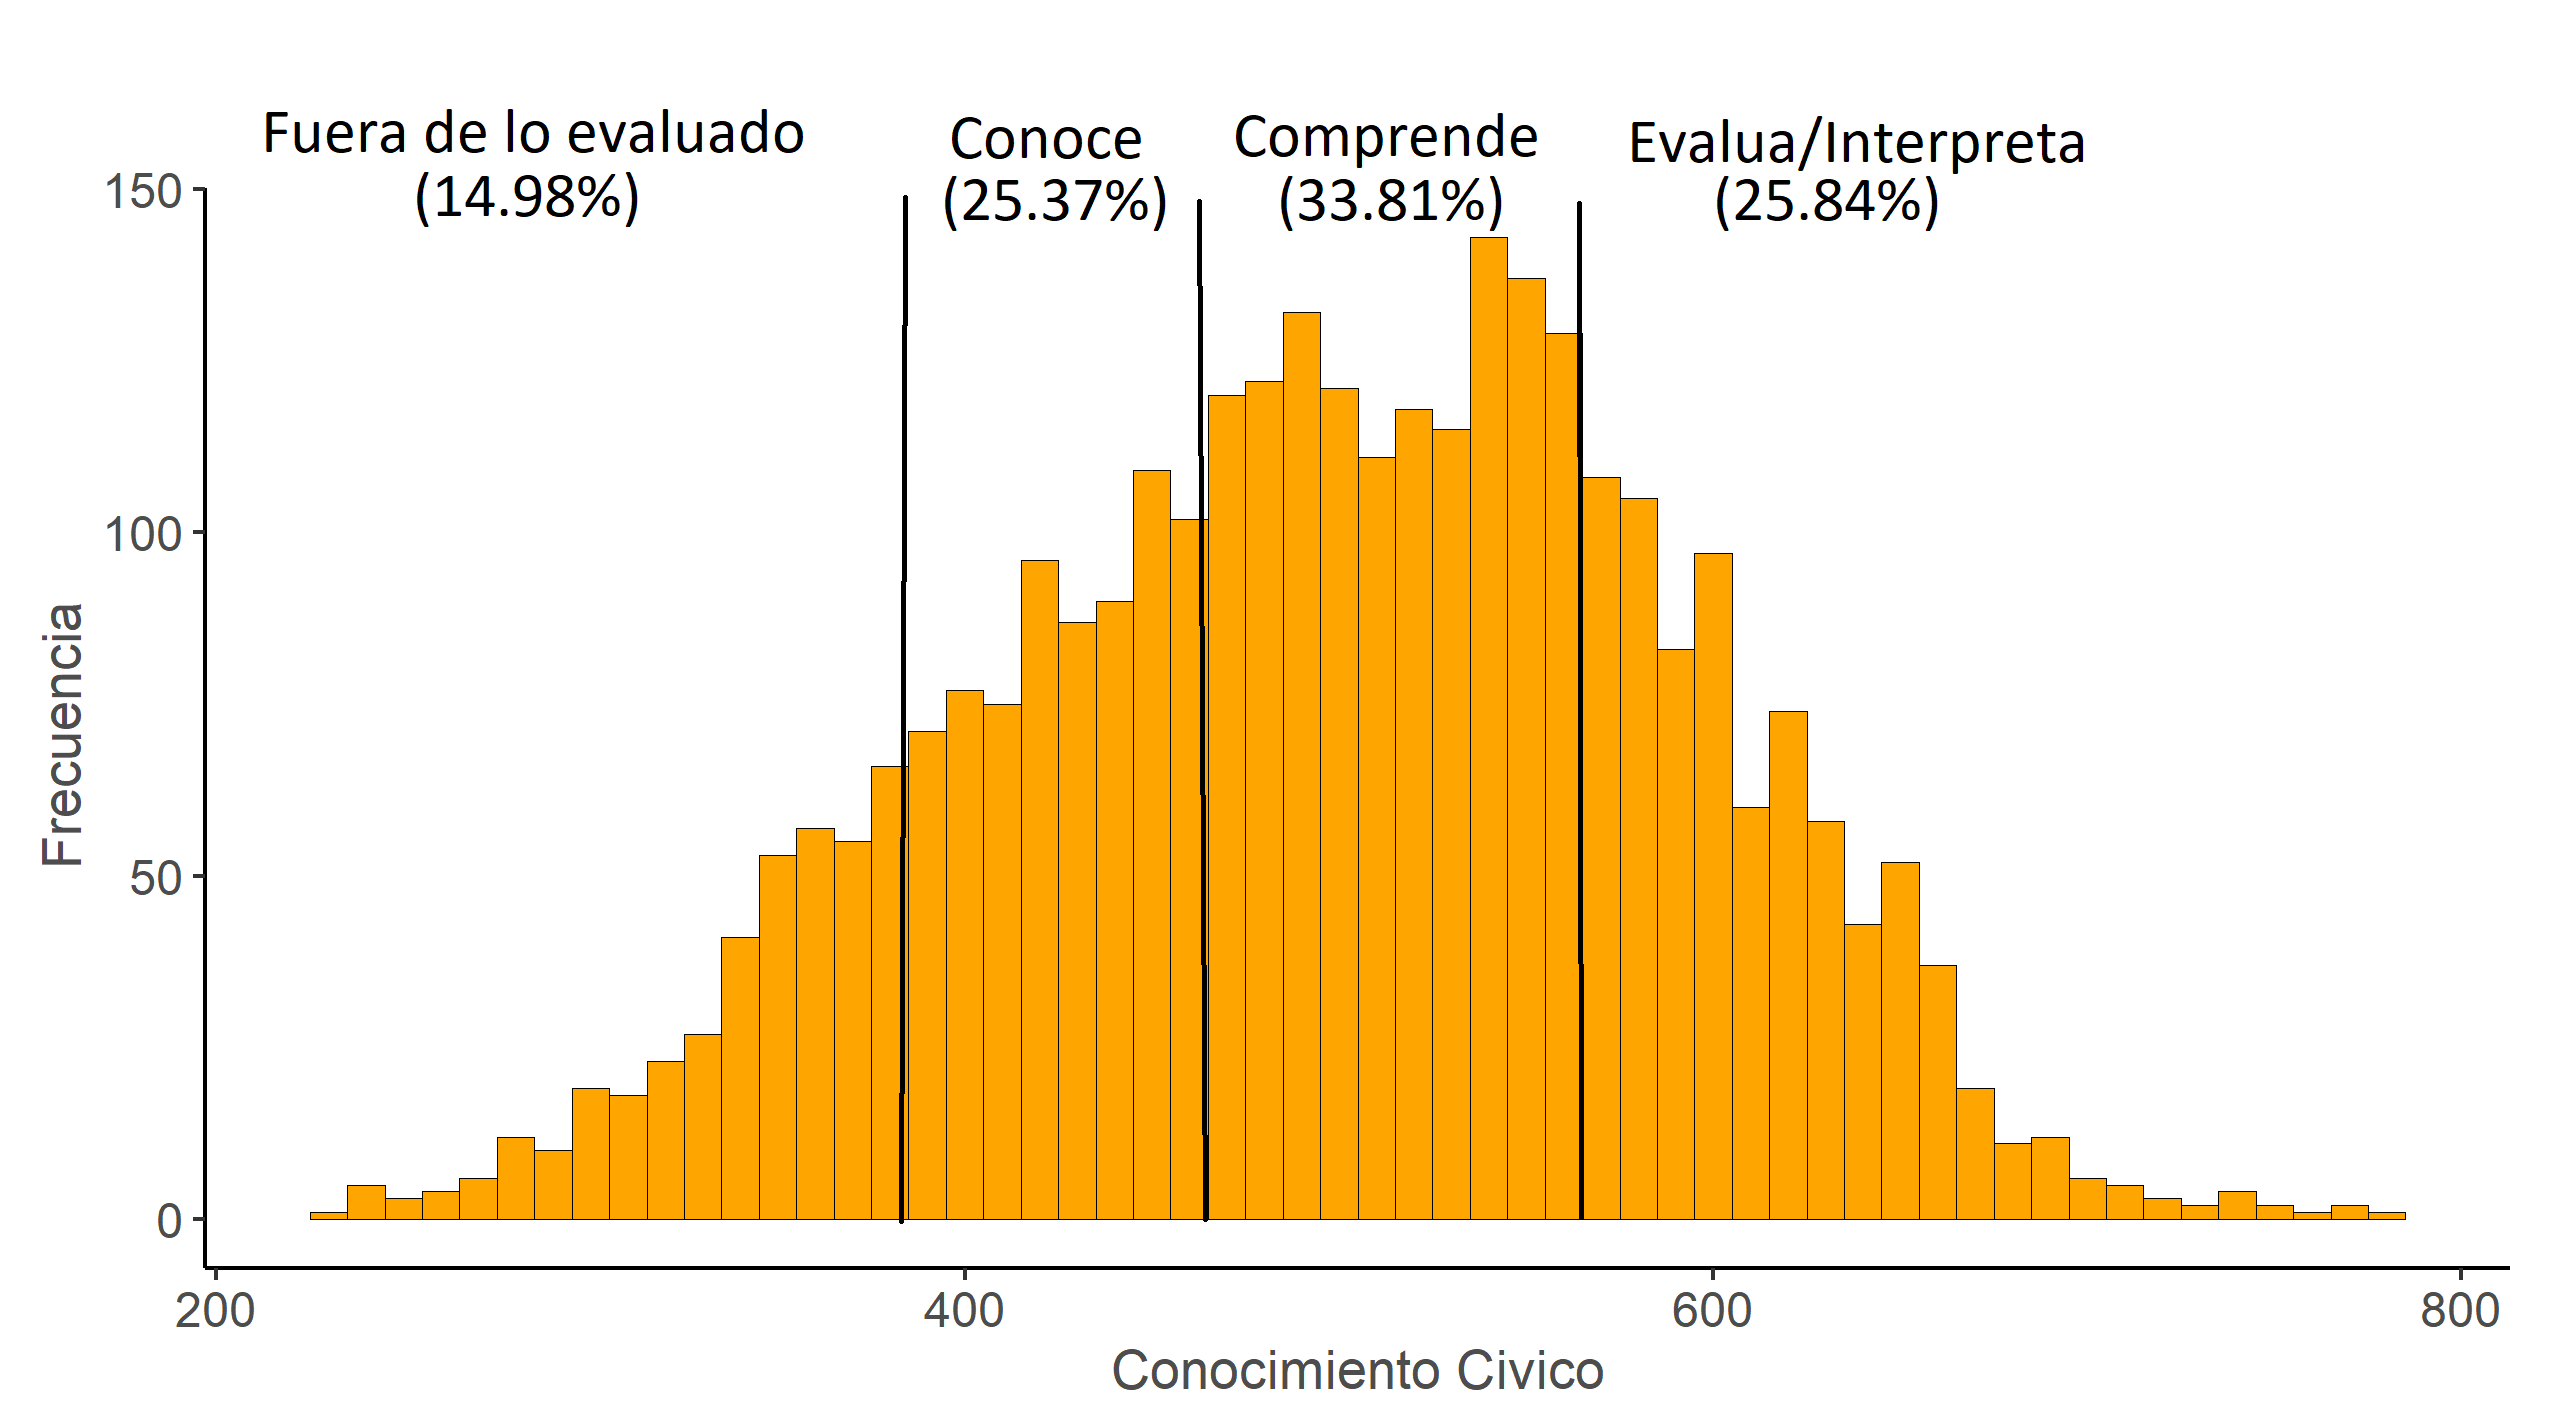
\includegraphics[width=1.1\linewidth]{images/dist} 

}

\caption{Distribución del Conocimiento Cívico}\label{fig:unnamed-chunk-6}
\end{figure}

\newpage

El grafico posterior corresponde a la distribución de la comprensión lectora, prueba en la cual se muestra un peor desempeño que en la prueba de conocimiento cívico. Dos de cada cinco estudiantes poseen una comprensión lectora insuficiente, mientras que menos de uno cada cuatro posee un nivel adecuado.

Esto da cuenta de un problema muy preocupante, ya que implica que buena parte de los estudiantes no poseen un desarrollo adecuado de habilidades como la comprensión, la interpretación o el análisis, habilidades las cuales hemos argumentado son fundamentales para la vida ciudadana.

\begin{figure}

{\centering 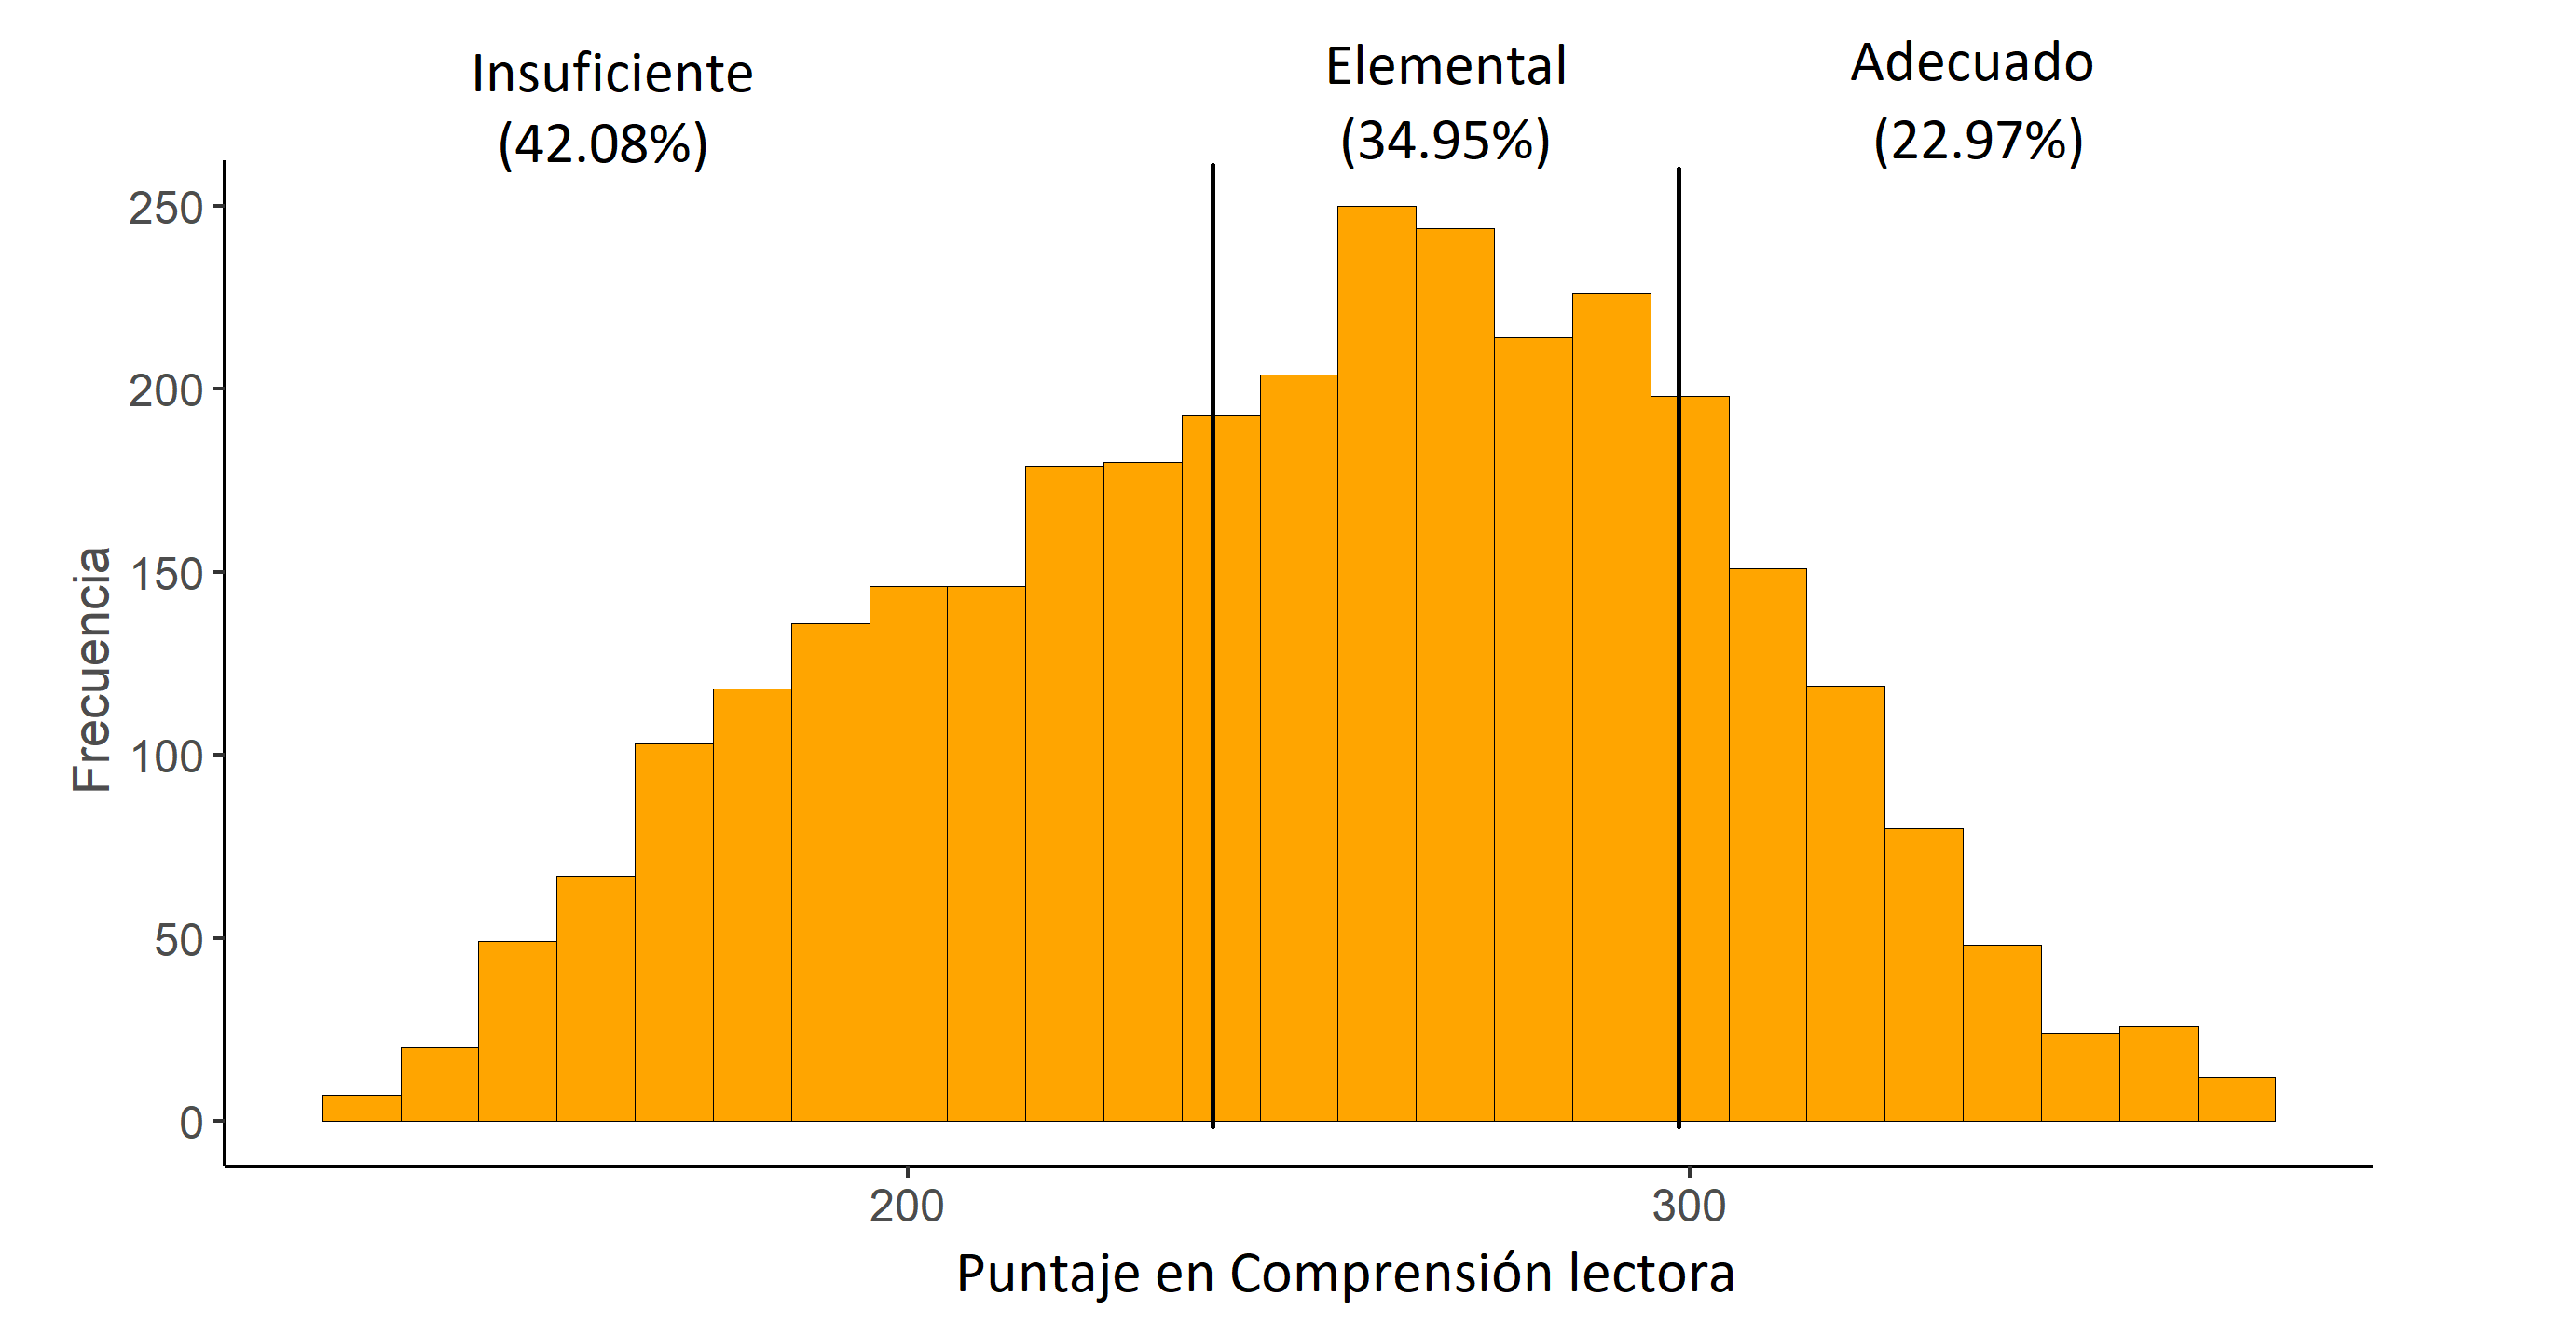
\includegraphics[width=1.1\linewidth]{images/dist2} 

}

\caption{Distribución de la Comprensión lectora}\label{fig:unnamed-chunk-7}
\end{figure}

\newpage

\hypertarget{anuxe1lisis-relacional}{%
\section{Análisis relacional}\label{anuxe1lisis-relacional}}

Retomando nuestra hipótesis y robusteciéndola con las definiciones planteadas, podemos decir que el manejo del lenguaje, como herramienta del razonamiento, posee una influencia positiva en las habilidades políticas necesarias para la vida ciudadana, entre las cuales destacan la comprensión, la interpretación y la evaluación. Igualmente podemos decir que ambos conceptos son bien medidos por la prueba de conocimiento cívico y ciudadano, así como por las pruebas de lectura. Antes de entrar en el trabajo de datos de esta investigación (que será con las bases ICCS y SIMCE), se presenta una evidencia preliminar.

A continuación, se puede observar un gráfico que expone la relación a nivel internacional, entre los promedios de los estudiantes por país de las pruebas de comprensión lectora de la prueba pisa y el conocimiento cívico de la ICCS.

\begin{figure}

{\centering 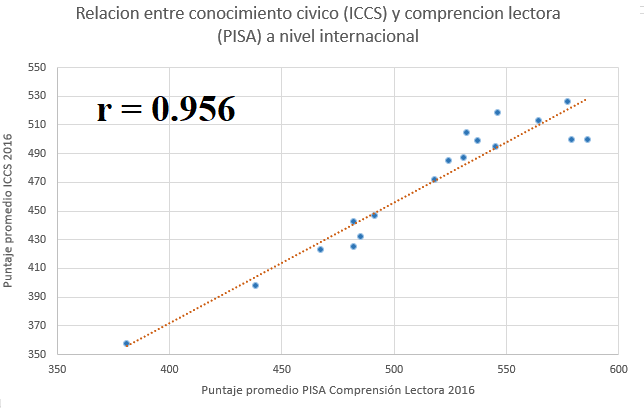
\includegraphics[width=1\linewidth]{images/relacionmacro} 

}

\caption{Relación internaciónal}\label{fig:unnamed-chunk-8}
\end{figure}

Como puede apreciarse, a nivel internacional, existe una estrecha relación entre ambas variables. Según esta relación, países con mayores niveles de comprensión lectora poseen igualmente mayores niveles de conocimiento cívico y ciudadano. Como se expone en la imagen, existe una relación de alta intensidad entre ambas variables (r = .95). No obstante, no hay que dejarse engañar por esta relación por dos razones. En primer lugar, esta relación no está controlada por ninguna variable. En segundo lugar, esta relación a nivel países, no nos permite afirmar que exista una relación entre comprensión lectora y conocimiento cívico a nivel individual o a nivel escuela. A continuación presentamos la relación entre el conocimiento cívico y la comprensión lectora en base a los datos individuales de la base ICCS-SIMCE.

\begin{figure}

{\centering 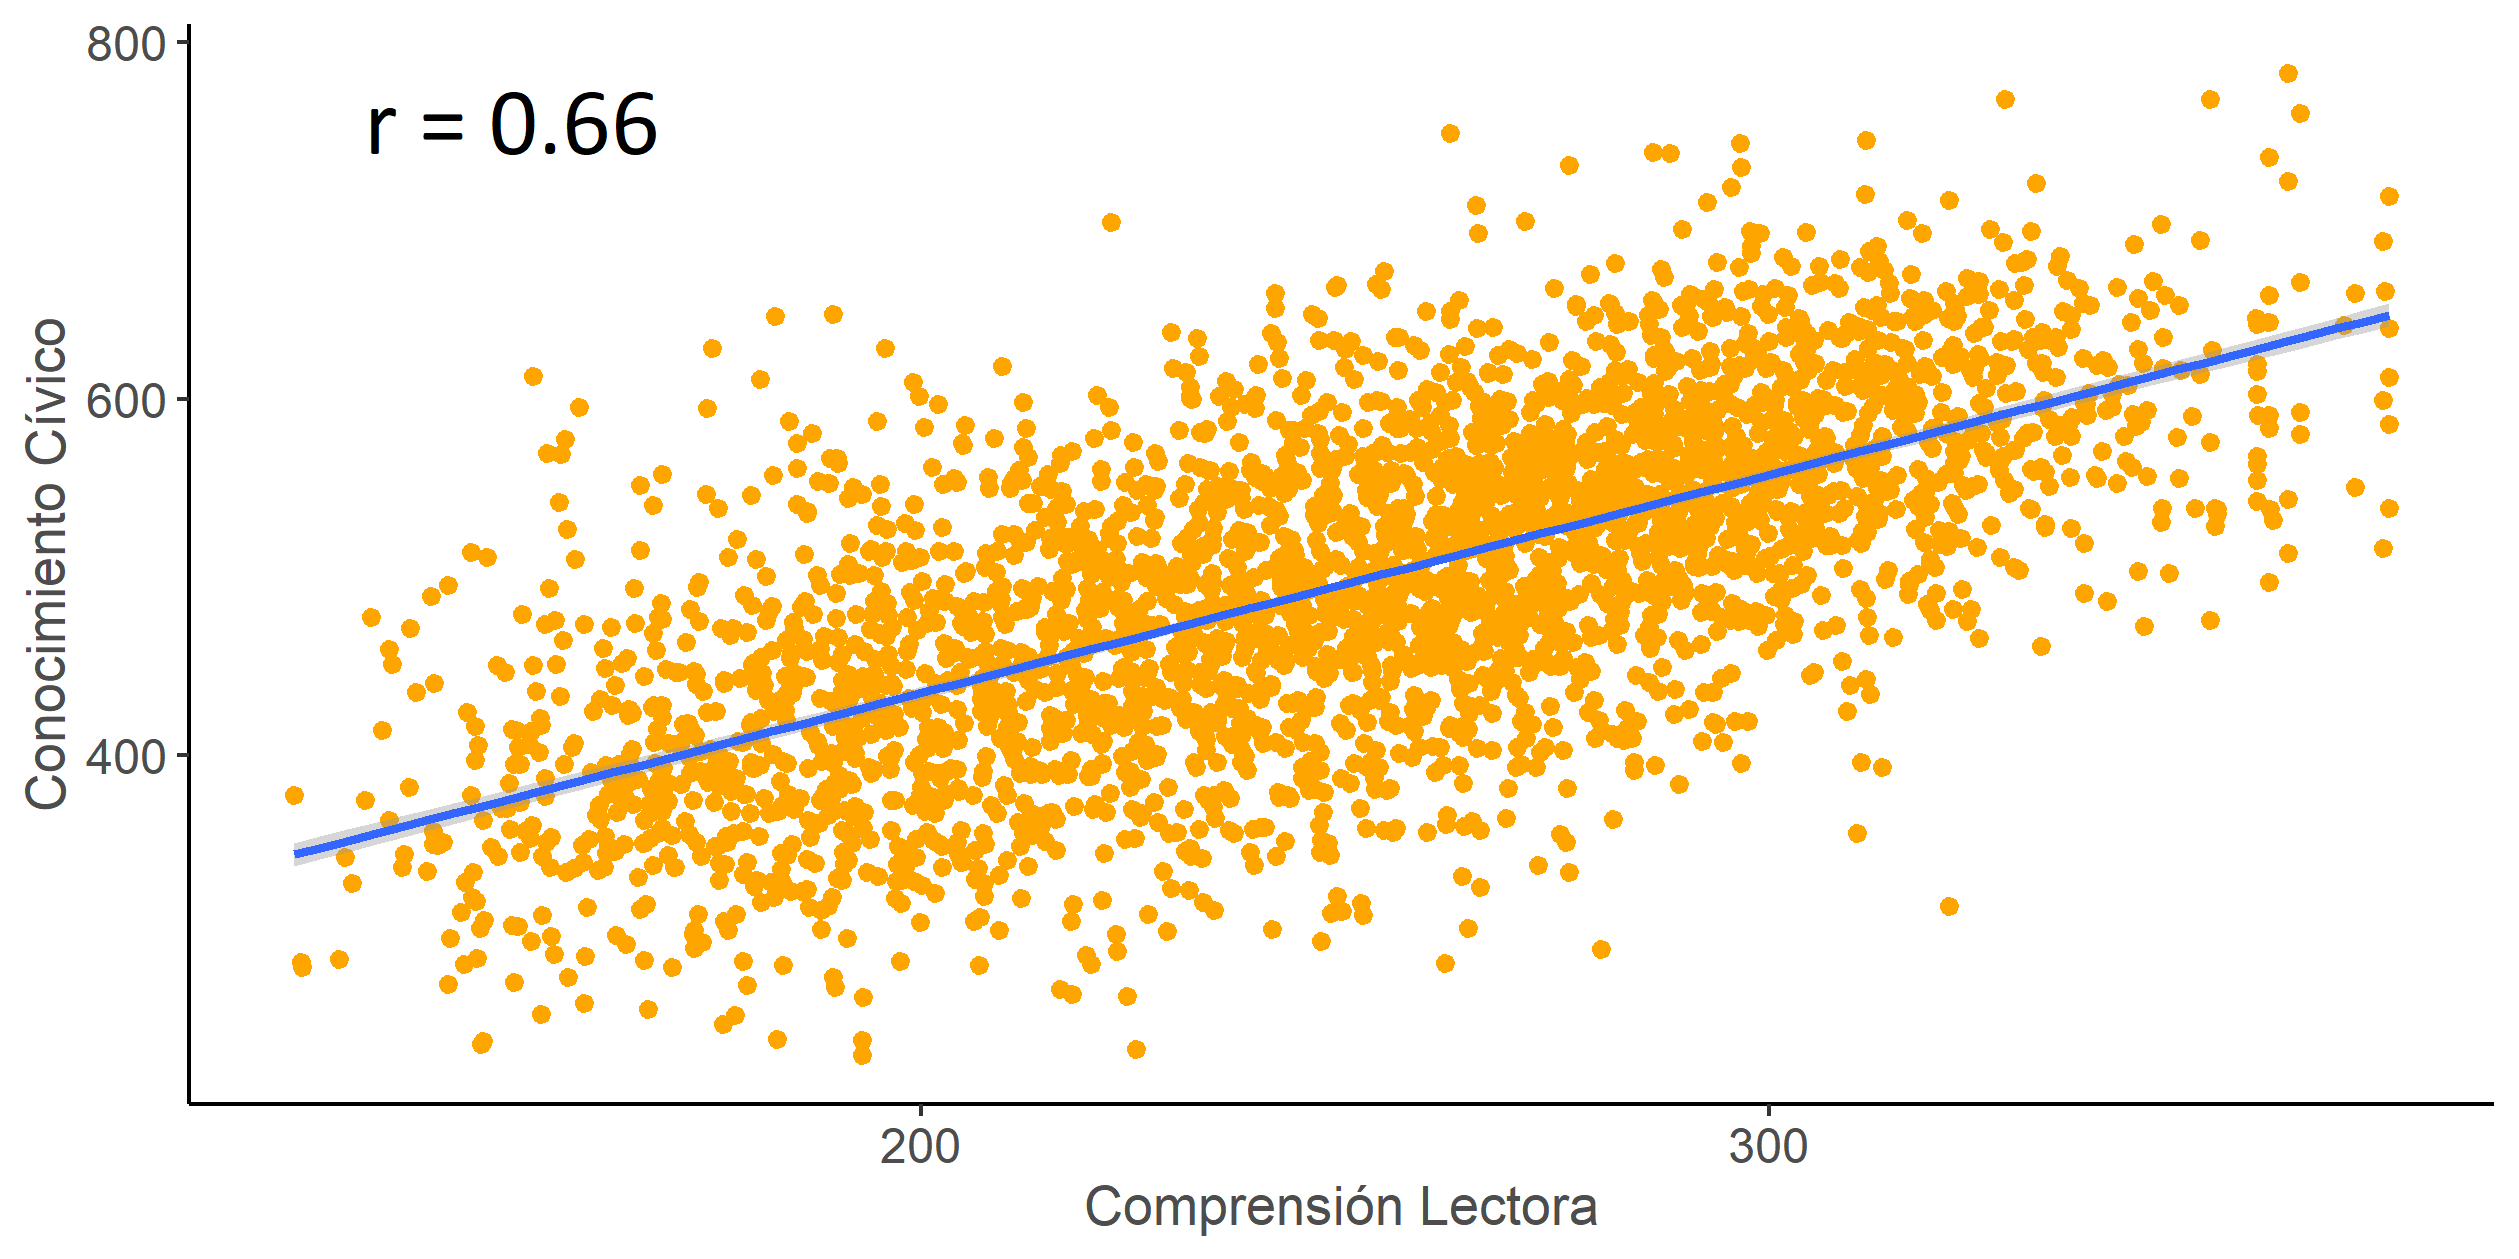
\includegraphics[width=0.8\linewidth]{images/scater} 

}

\caption{Grafico de disperción}\label{fig:unnamed-chunk-9}
\end{figure}

Como puede verse la relación es igualmente positiva, aunque, en relación a lo internacional, disminuye la intensidad De todos modos, se puede apreciar en base a la correlación de Pearson una relación de alta intensidad según los parámetros de Cohen (\(r= .66\)).

\begin{figure}

{\centering 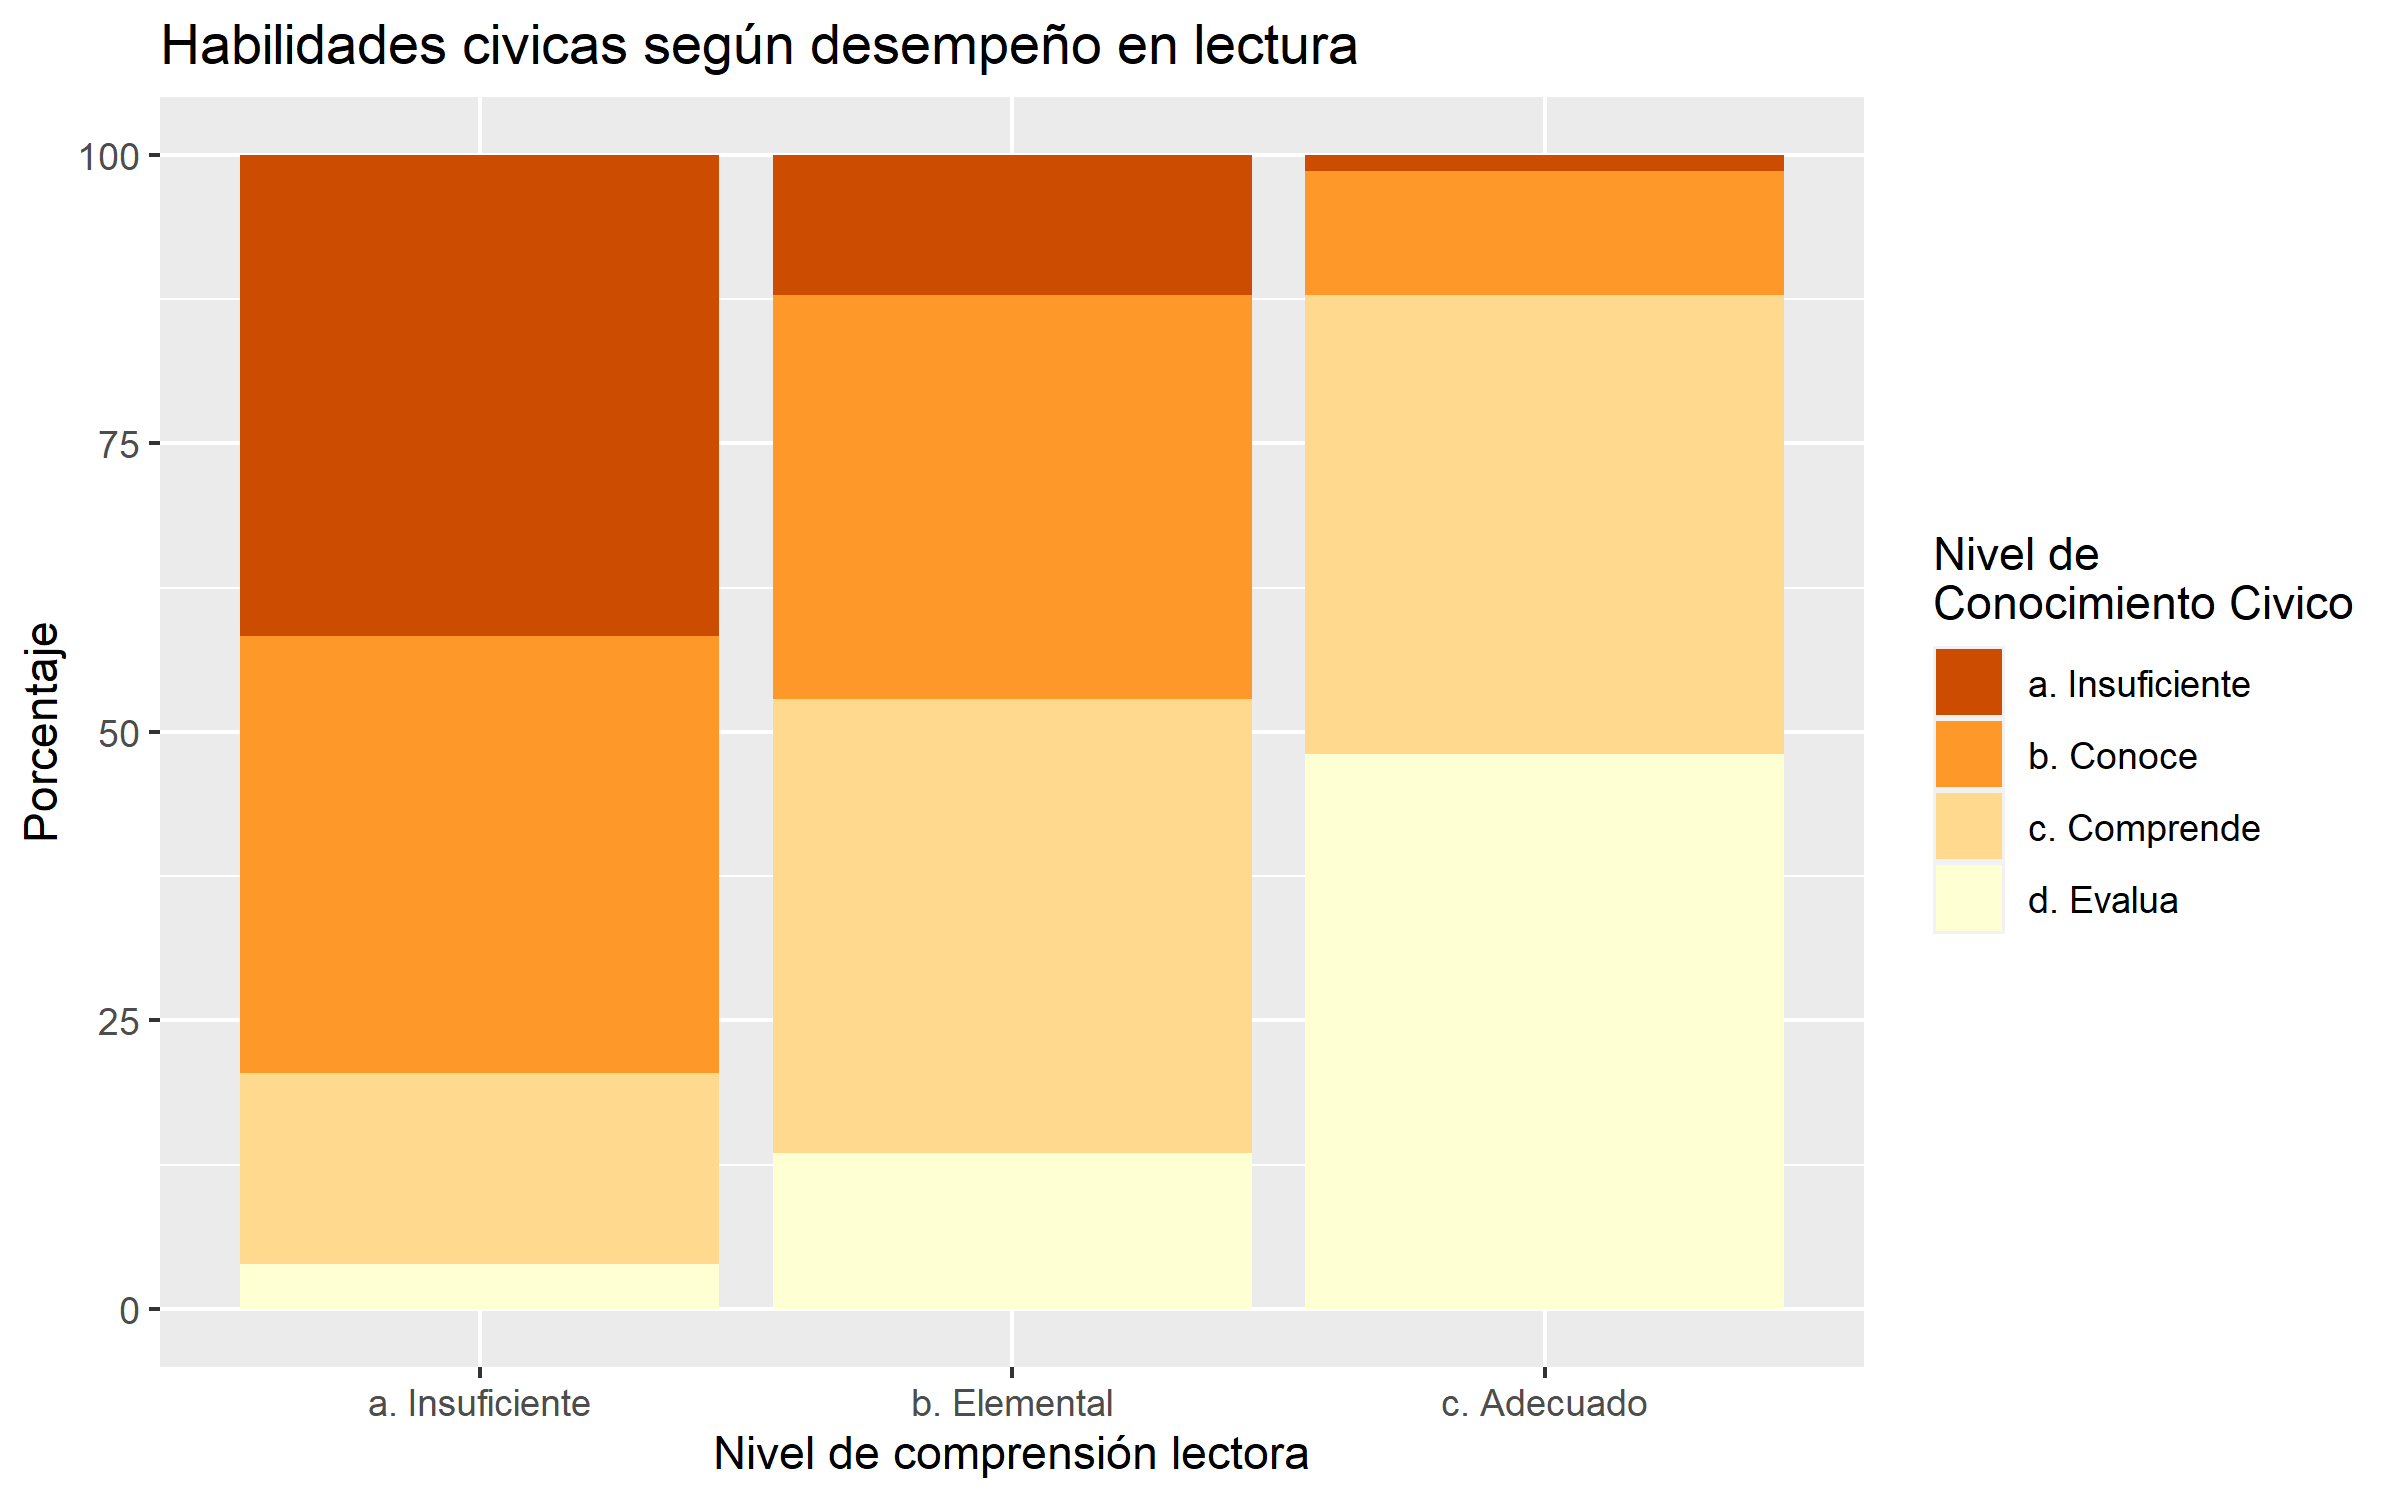
\includegraphics[width=0.8\linewidth]{images/graficobivariadocategorico} 

}

\caption{Niveles de conocimiento cívico según comprensión lectora}\label{fig:unnamed-chunk-11}
\end{figure}

El grafico de la figura número 9.5, resulta sumamente ilustrativo del punto que busca señalar esta tesis. Para entender el grafico debemos comprender que se está graficando la relación entre los niveles de conocimiento cívico y los niveles de manejo del lenguaje. Los niveles de manejo del lenguaje se clasifican en insuficiente, elemental y adecuado, mientras que los niveles de conocimiento cívico no refieren a que tan aceptable son los resultados, sino hasta que habilidad logran desarrollar los estudiantes en la prueba de formación ciudadana. Como se mencionó anteriormente para responder bien la prueba de cívica no solo es necesario poseer un amplio conocimiento de memoria sobre asuntos cívicos y ciudadanos. Más bien es necesario tener habilidades para poder interpretar situaciones políticas. Al respecto la habilidad más compleja es la de evaluar, la cual puede comprenderse según los evaluadores como dar cuenta de la postura de un enunciado o evaluar críticamente su pertinencia en determinada situación. Analicemos minuciosamente la distribución de cada uno de los conjuntos de barras.

El primer conjunto de barras refiere a las personas que son calificadas como insuficientes en la prueba de conocimiento cívico. Esta clasificación es bastante deprimente, pues implica que esos estudiantes no poseen el nivel mínimo que busca medir la prueba. Por decirlo así, quedan por debajo de la regla de medición. Como vimos anteriormente aproximadamente el 15\% de los estudiantes se encuentra en esta categoría. Entre ellos, es notorio, observando los colores que prácticamente se trata de estudiantes con niveles deficientes de manejo del lenguaje. Casi todos los que pertenecen a este grupo comparten la característica de poseen una mala calificación en la prueba de comprensión lectora. Esto va en línea con nuestra hipótesis.

El segundo grupo corresponde a quienes logran demostrar sus conocimientos en la prueba, pero no sus habilidades. En este grupo siguen siendo preminentes los estudiantes que poseen un nivel menor al elemental en comprensión lectora. Además, se puede observar que existe una mayor proporción de estudiantes que poseen simplemente un nivel elemental de lectura pero que no es adecuado para su grado de estudio.

En el tercer grupo se encuentran quienes demostraron poseer la capacidad de comprender situaciones políticas. Esta es una habilidad fundamental para el mundo político, pues comprenderlo es parte esencial del proceso para participar de él. En este grupo, la mayoría de los estudiantes poseen un nivel de lectura elemental, pero no adecuado para su nivel. Seguidamente, el grupo que más destaca después del elemental es quienes poseen un nivel insuficiente manejo del lenguaje. Finalmente, en este grupo a diferencia de los dos anteriores es más considerable la proporción de estudiantes que poseen un nivel adecuado, mas no sobresaliente. Quizás sería bueno para versiones posteriores incluir la categoría sobresaliente en lenguaje.

El último grupo corresponde a quienes poseen la habilidad de interpretar y evaluar situaciones políticas. Esta es una habilidad de alta exigencia cognitiva y requiere el manejo de las habilidades anteriores. Una persona que es capaz de interpretar y evaluar propuestas políticas está mucho más preparada para la ciudadanía, especialmente desde una perspectiva del actor crítico, pues tendrá herramientas para esa crítica. Es este en el único grupo que se encuentra una prevalencia de las personas con una lectura adecuada y el único grupo donde la presencia de estudiantes con una lectura deficiente es casi marginal. De todos modos, resulta interesante profundizar en aquellos casos que logran poseen habilidades de evaluación sin un buen manejo del lenguaje.

Lo evidenciado en esta descripción de los datos va en dirección de lo planteado en las hipótesis. Mientras mejores son las habilidades lingüísticas del estudiante, más probable parece ser que este posea buenas habilidades para la vida cívica y ciudadana. Para comprobar estos resultados preliminares recurriremos las regresiones multinivel que responden mejor a las condiciones de los datos a analizar.

\hypertarget{modelos}{%
\section{Modelos}\label{modelos}}

\hypertarget{anuxe1lisis-multinivel-varianza-entre-escuelas}{%
\subsection{Análisis Multinivel: Varianza entre escuelas}\label{anuxe1lisis-multinivel-varianza-entre-escuelas}}

A partir del modelo nulo, utilizando la varianza entre grupos y residual, se cálculo la correlación intraclase, es decir, la proporción de la varianza del conocimiento cívico que es explicada por el nivel escuela. Prácticamente un tercio de la varianza del conocimiento cívico depende del nivel escolar y agregado, lo que da cuenta de la importancia de controlar por estas variables así como de investigar que cualidades de la escuela fomentan el conocimiento cívico.

\begin{figure}

{\centering 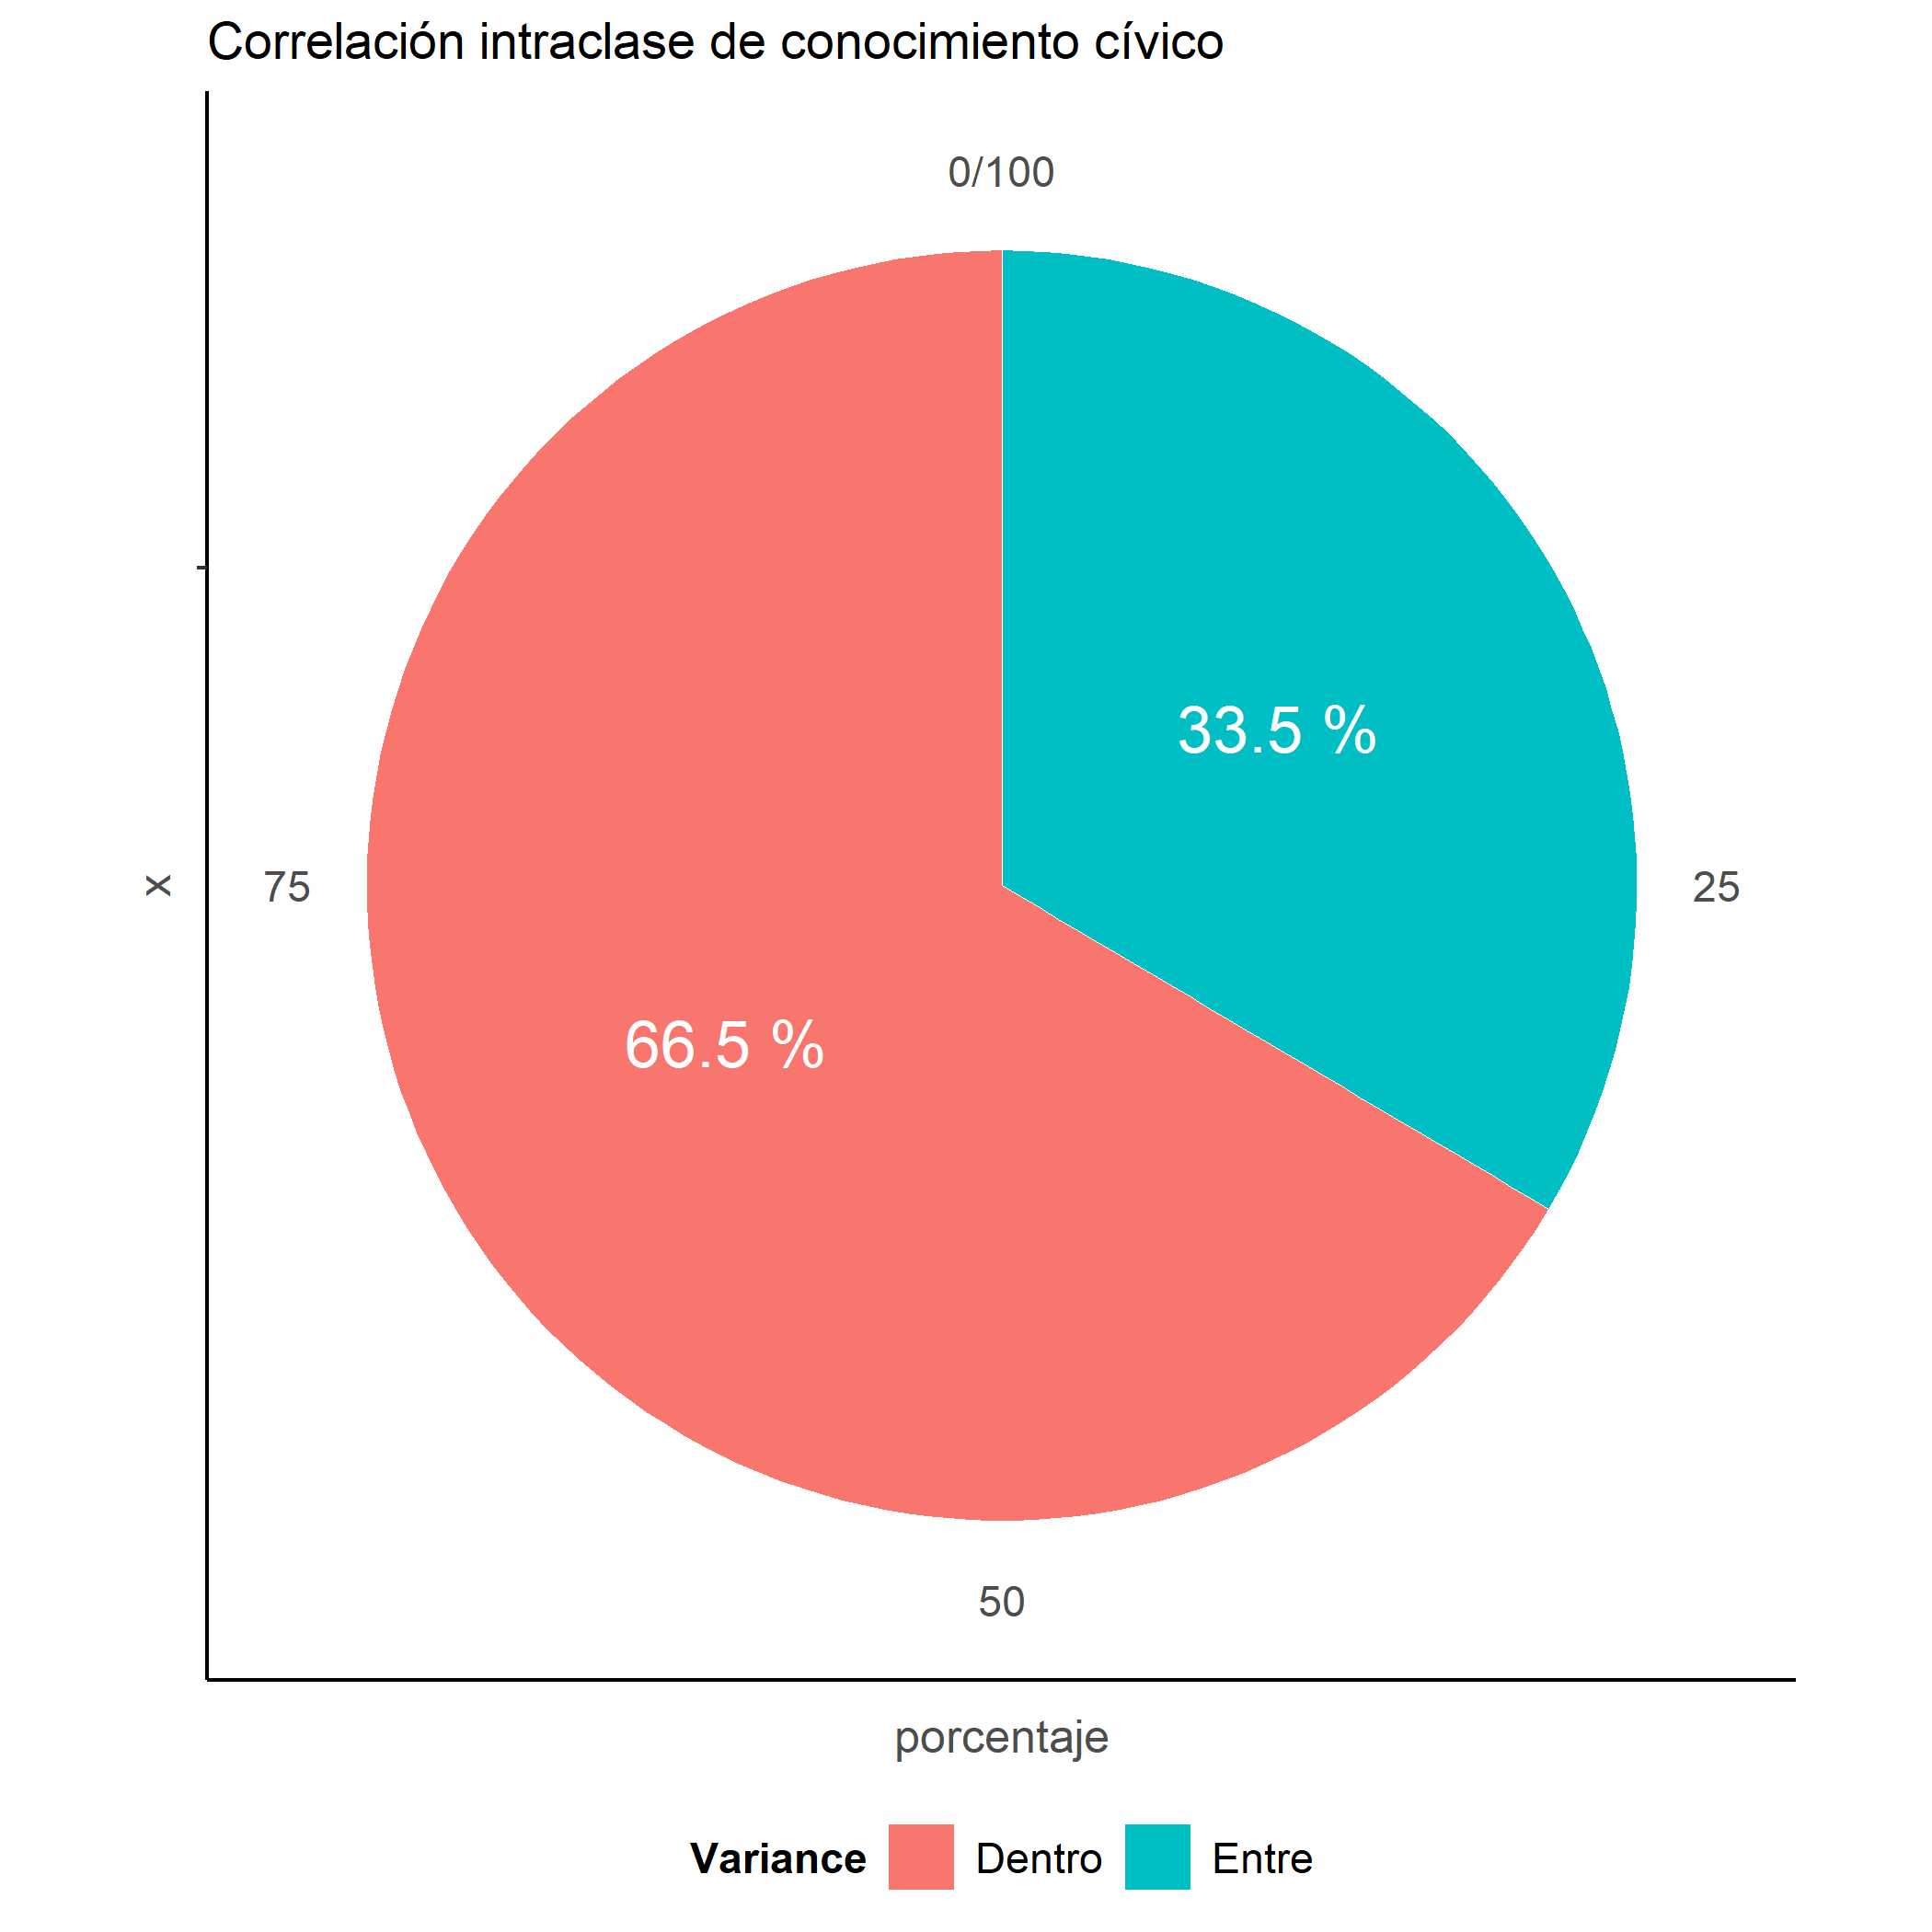
\includegraphics[width=0.5\linewidth]{images/iccplot} 

}

\caption{Proporción de varianza entre y dentro}\label{fig:unnamed-chunk-12}
\end{figure}

\newpage

\hypertarget{resultados-del-anuxe1lisis-multinivel-efectos-e-interacciuxf3n.}{%
\subsection{Resultados del análisis multinivel: efectos e interacción.}\label{resultados-del-anuxe1lisis-multinivel-efectos-e-interacciuxf3n.}}

En la tabla consecutiva se presentan 3 modelos multinivel. El primer modelo evalúa la propuesta de esta tesis, la asociación entre Conocimiento Cívico y Comprensión Lectora. El segundo modelo expone las variables señaladas por la literatura para explicar. Por último, el tercer modelo evalúa si el efecto de la comprensión lectora es controlado por otras variables relevantes como el origen del estudiante, sus intereses y las practicas escolares.

\begin{center}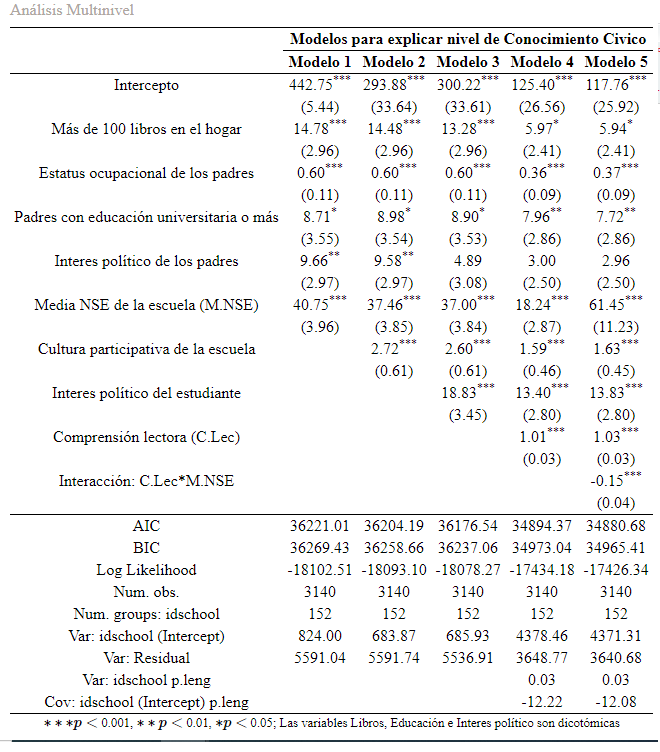
\includegraphics[width=0.8\linewidth]{images/regmultinivel} \end{center}

El primer modelo nos permite evidenciar la asociación entre comprensión lectora y conocimiento cívico. El efecto es significativo con un 99\% de confianza. Por cada punto que aumenta la comprensión lectora, aumenta un punto el conocimiento cívico. La fuerza de la relación es considerablemente alta. A nivel escuelas prácticamente el 60\% de la varianza del conocimiento cívico es explicada por las diferencias en comprensión lectora. A nivel estudiante, el 34\% de la varianza es explicada por la comprensión lectora. En suma, la comprensión lectora tiene un potencial explicativo sobre las diferencias entre las escuelas y entre los estudiantes sobre conocimiento cívico.

El segundo modelo presenta el efecto de las variables consideradas relevantes por la literatura. En general poseen un efecto de gran tamaño. Tener más de 100 libros en el hogar implica 13 puntos más en la prueba de conocimiento cívico con un 99\%. El modelo que incluye teoría de recursos y de socialización es muy efectivo para explicar las diferencias entre escuelas, explicando un 76\% de ellas. No obstante, es muy incapaz de explicar diferencias entre estudiantes de un mismo contexto, pues solo explica el 4\% de la varianza dentro de las escuelas.

El tercer modelo incluye tanto la propuesta teórica de esta tesis como los efectos destacados anteriormente por el campo de investigación, permitiendo controlarlos. Como se puede ver el efecto de la comprensión lectora se mantiene más o menos igual al incluir todas las variables de origen económico y socialización política, dando cuenta que es una relación robusta frente a otras explicaciones. También se puede apreciar como son controladas las variables de origen familiar, el efecto de tener libros en el hogar y el del estatus ocupacional de los padres disminuye a la mitad. Esto indica que parte del efecto del origen social se podría explicar por la trasmisión de ventajas para desarrollar la comprensión lectora. Este modelo final posee una gran capacidad explicativa a nivel 2 explicando el 87\% de la varianza del conocimiento cívico y un 35\% de la varianza entre estudiantes.

En suma, se puede ver que la comprensión lectora posee un efecto significativo de gran intensidad sobre la comprensión lectora. Incorporar la comprensión lectora agrega una buena proporción de varianza explicada, especialmente a nivel estudiantes, que es donde más hay varianza y los otros modelos no habían podido explicarla. Además, este efecto se mantiene al controlar por variables de origen, más aún, es capas de controlar buena parte de sus efectos, lo cual profundizaremos a continuación con los análisis de medicación multinivel.

\hypertarget{resultados-de-la-mediaciuxf3n-multinivel.}{%
\subsection{Resultados de la mediación multinivel.}\label{resultados-de-la-mediaciuxf3n-multinivel.}}

A continuación, se presentan los resultados del análisis de mediación multinivel. En estos se evalúa la capacidad del lenguaje de explicar la relación entre NSE y conocimiento cívico, haciendo esta evaluación a nivel uno y nivel dos como recomienda la literatura. Para este fin, se evalúa primero, si el NSE se relaciona con lenguaje, luego si el NSE se relaciona con el conocimiento cívico y, posteriormente, si es que el efecto de NSE sobre conocimiento cívico es controlado por la comprensión lectora, repitiendo este proceso en ambos niveles. En la siguiente tabla el nombre de la columna indica la variable dependiente.

\begin{center}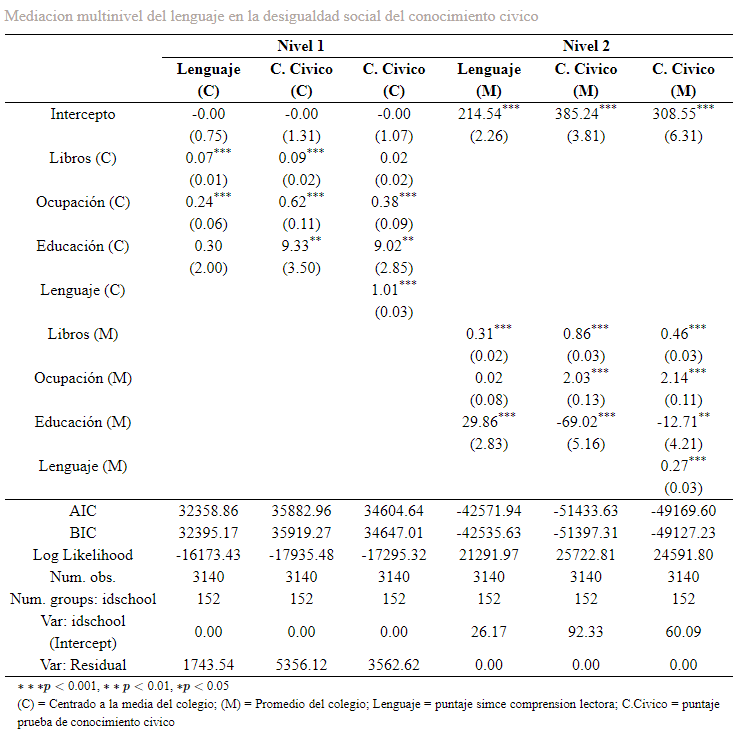
\includegraphics[width=0.8\linewidth]{images/Mediacion_n1n2} \end{center}

A partir de los resultados de la tabla anterior, es posible concluir que la comprensión lectora posee la capacidad de explicar parcialmente la desigualdad en el conocimiento cívico. En primer lugar, en torno al nivel uno, podemos ver que el lenguaje es influido por la cantidad de libros en el hogar y la ocupación de los padres, pero no la educación de los padres. Seguidamente se constata que las tres variables afectan el conocimiento cívico y que, al incluir el manejo del lenguaje como control, desaparece completamente el efecto de tener libros en el hogar, esto es un descubrimiento interesante considerando el rol que ha tenido esta variable para explicar el conocimiento cívico. Además el efecto de la ocupación es controlado en un 38\%, lo cual es comprensible, de modo tal que parte del efecto de la ocupación de los padres se debe a que fomenta, ya sea por socialización o recursos, un mejor manejo del lenguaje, como señalaba Bernstein. Curiosamente el efecto de tener padres con nivel universitario no es controlado por el lenguaje.

A nivel dos, se puede ver que la cantidad de libros promedio del hogar y la proporción de padres universitarios poseen un efecto en el promedio de la comprensión del lenguaje. Seguidamente, se puede ver que todas las variables de recursos afectan el promedio de conocimiento cívico, aunque resulta extraño el efecto negativo que posee la proporción de padres universitarios. Al incluir el control por el promedio de puntaje en lenguaje del colegio, la variable agregada de los libros disminuye su efecto al igual que la variable de educación de los padres. No obstante, no se logra controlar el efecto del estatus ocupacional promedio de los padres.

\hypertarget{conclusiones}{%
\chapter{Conclusiones}\label{conclusiones}}

En consideración de los resultados, podemos entregar algunas respuestas parciales a nuestros objetivos de investigación.

En primer lugar, podemos decir que existe una relación moderadamente alta entre el conocimiento Cívico y la comprensión lectora relación la cual no solo se mantiene al incluir otras variables fundamentales en el modelo, sino que es capaz de controlar buena parte del efecto de las variables de origen social. La evidencia del efecto de la comprensión lectora, no niega el efecto positivo sobre el conocimiento Cívico que pueden tener variables como la cultura democrática del establecimiento, lo cual se evidencia con la mantención de este efecto al controlar por comprensión lectora.

En segundo lugar, en función de los resultados, podemos decir que aquellas teorías que explicaban la relación entre NSE y conocimiento cívico, por la transmisión de valores, si bien son ciertas, poseen una visión parcial de lo que ocurre ya que en buena medida la desigualdad social del conocimiento cívico se relaciona ampliamente con la desigualdad social de la comprensión lectora, la cual se relaciona con el capital cultural objetivado de los padres (más de 100 libros en el hogar) y el acceder a buena educación. Es decir, no es tanto que los padres adinerados eduquen democráticamente a sus hijos, sino que más bien, ya sea por transmisión directa o por acceso a buena educación, les otorgan un mayor manejo del lenguaje, lo cual les permite igualmente incorporar de manera más compleja la realidad política, teniendo más herramientas para comprender, analizar y criticar políticamente.

En tercer lugar, gracias a la evidencia, podemos señalar que la comprensión lectora puede ser una forma de mejorar el conocimiento Cívico en sectores vulnerables, puesto que estudiantes de dichos sectores que si poseen un buen manejo del lenguaje poseen igualmente altas capacidades y conocimientos para la vida ciudadana. En función de lo anterior, se hace necesario estudiar experimentalmente el efecto que podría tener un reforzamiento en lenguaje para la prueba de la ICCS.

\hypertarget{discusiuxf3n}{%
\section{Discusión}\label{discusiuxf3n}}

Dados los resultados, y el rol prominente de la comprensión lectora en el conocimiento Cívico, se hace necesario revisar algunas propuestas que intentan explicar el conocimiento Cívico, puesto que pueden caer en resultados espurios al no considerar una variable relevante dentro de sus modelos.

En términos teóricos esta investigación ayuda a profundizar la comprensión de la reproducción social de la desigualdad política, como \citet{brady_Political_2015} sugerían necesario para avanzar en este campo. Estos resultados evidencias que las diferencias sociales en habilidades políticas, no se deben tanto a la transmisión de valores democráticos, como a la transmisión de habilidades relacionadas con el manejo del lenguaje.

Igualmente, se hace necesario profundizar hasta qué punto la comprensión lectora es necesaria para la vida política o más bien es un problema de error de medida, en el cual se incorpora varianza no deseada a la escala. En consideración de lo anterior, es posible que, al generar instrumentos con menores niveles de abstracción en la redacción de las situaciones y preguntas, se generen menores diferencias de conocimiento Cívico entre distintos grupos sociales.

En comparación a otros modelos teóricos esta propuesta es muy efectiva para explicar las diferencias entre los estudiantes de un mismo contexto. Incorporar esto nos permite mirar más allá y más profundamente las desigualdades sociales en el conocimiento cívico.

Respecto a cuáles son los caminos que deben tomarse para mejorar la desigualdad en el conocimiento cívico y en la participación ciudadana, resulta evidente después de los resultados, que además de reforzar la educación cívica en los colegios como ya se está haciendo (y debe seguirse haciendo, debe fomentarse la comprensión lectora). Incluso podemos decir que cuando se posee altos niveles de comprensión lectora, las diferencias de estatus socioeconómico no afectan de manera sustancial, existiendo estudiantes de colegios con bajo nivel económico que poseen una buena comprensión lectora y cívica. Al respecto, tipos de clases que impliquen lectura colectiva y discusión sobre lo leído, para entender en conjunto el sentido de los textos, puede ser una muy buena estrategia, puesto que está demostrado que los profesores que realizan dichas actividades mejoran el puntaje en lenguaje de sus estudiantes (Lorena Ortega) así como que aulas más participativas poseen un efecto para el conocimiento cívico. Es en dichos espacios de participación donde puede sacarse el provecho al capital cultural de cada estudiante y fomentar el efecto par.

En relación al nuevo plan de formación ciudadana, y considerando estos resultados es sensato esperar un efecto diferencial de la política en cada establecimiento según el nivel de comprensión lectora del colegio, lo cual está relacionado con el nivel socioeconómico. Quizás sea prudente en miras del objetivo de la política, prestar ayuda especializada a colegios que posean bajos niveles de comprensión lectora. Dentro de los colegios prestar apoyo a los estudiantes con dificultades al respecto también puede ser una buena medida a aplicar en cursos anteriores al último ciclo de tercero cuarto, donde deberán aplicar dichas habilidades en la reflexión ciudadana y en la incorporación de conocimientos cívicos.

El considerar que la comprensión de la vida cívica puede estar asociada a la comprensión del lenguaje no solo es relevante dentro del campo de la educación, sino también en el campo de la acción política y la democracia. Si un joven es capaz de comprender mediante el lenguaje distintos ideales democráticos es más probable que actúe y opine en concordancia con ellos. Más aun, el comprender distintos ideales puede abrir las posibilidades de acción del sujeto ya que, si la realidad es social y construida mediante el lenguaje, poseer un mayor manejo del lenguaje implica una mayor capacidad reflexiva sobre la realidad, una mayor capacidad crítica y, por ende, una mayor capacidad de agencia. El lenguaje no solo nos permite enunciar el mundo, sino que también nos ayuda a analizarlo, criticarlo y así actuar reflexivamente sobre él.

Además, evidenciar el rol del lenguaje en el conocimiento cívico puede ser muy provechoso para las políticas públicas, ya que contar con información del contexto de aplicación del nuevo curso de formación ciudadana nos permite anticiparnos a sus posibles obstáculos. En primer lugar, podríamos suponer que la aplicación de un nuevo ramo de educación cívica, en el contexto de un socialmente desigual manejo del lenguaje, podría incrementar las brechas sociales en la materia, dado que los colegios de mayor nivel socioeconómico poseen un mayor manejo del lenguaje y por ello se encuentran en mejores condiciones para incorporar los conocimientos cívicos. En consideración de esta posibilidad, seria provechoso para el objetivo del ramo, realizar planes de reforzamiento colectivo en lenguaje para aquellos colegios que poseen menores indicadores en las pruebas estandarizadas de comprensión lectora. En consideración del mismo argumento y considerando las inequidades dentro de los estudiantes de un mismo curso, podría ser provechoso prestar asistencia psicopedagógica a estudiantes que posean un menor manejo del lenguaje, antes de que estos se enfrenten en el último ciclo de educación a la formación ciudadana. Para evaluar estas medidas, es necesario comprobar la capacidad que posee el lenguaje para disminuir la desigualdad de habilidades políticas.

\begin{Shaded}
\begin{Highlighting}[]
\CommentTok{\#* la desigualdad educativa como barrera para la igualdad politica. }
\CommentTok{\# podriamos confundir un colegio bueno en lenguaje por uno bueno en civica.}
\end{Highlighting}
\end{Shaded}

\hypertarget{bibliografuxeda}{%
\chapter*{Bibliografía}\label{bibliografuxeda}}
\addcontentsline{toc}{chapter}{Bibliografía}

% %%%%%%%%%%%%%%%%%%%%%%%%%%%%%%%%%%%%%%%%%%%%%%%%%
% %%% Bibliography                              %%%
% %%%%%%%%%%%%%%%%%%%%%%%%%%%%%%%%%%%%%%%%%%%%%%%%%
% \addtocontents{toc}{\vspace{.5\baselineskip}}
% \cleardoublepage
% \phantomsection
% \addcontentsline{toc}{chapter}{\protect\numberline{}{Bibliography}}
\bibliography{tesis}

%% All books from our library (SfS) are already in a BiBTeX file
%% (Assbib). You can use Assbib combined with your personal BiBTeX file:
%% \bibliography{Myreferences,Assbib}. Of course, this will only work on
%% the computers at SfS, unless you copy the Assbib file
%%  --> /u/sfs/bib/Assbib.bib



\end{document}
